%\documentclass{beamer}

%\mode<presentation> {
%\usetheme{Madrid}
%}
\documentclass[a4paper,12pt]{article}
\usepackage{gensymb}
\usepackage[english]{babel}
\usepackage{graphicx} % Allows including images
\usepackage{colortbl} % Allows the use of \toprule, \midrule and \bottomrule in tables
\usepackage{booktabs}
\usepackage{caption}
\begin{document}

\begin{figure}
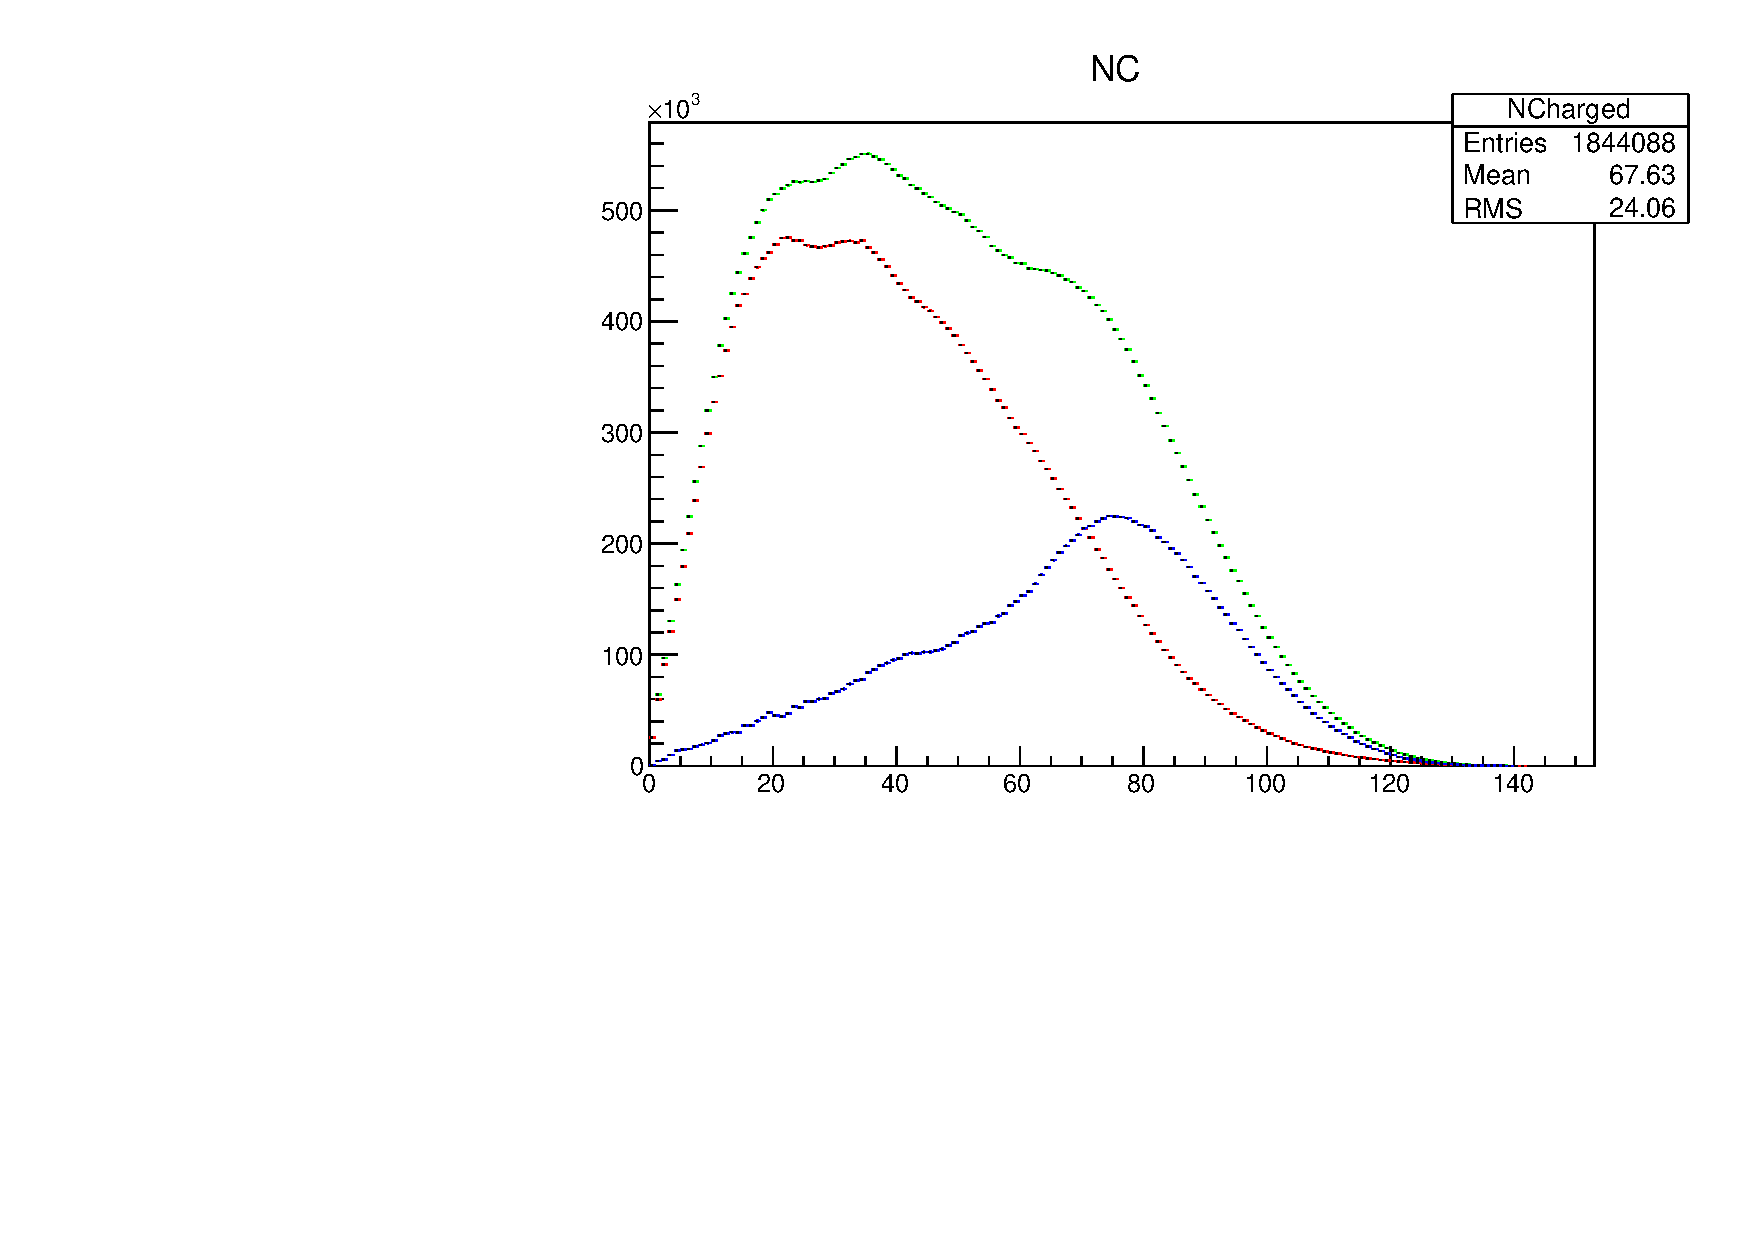
\includegraphics[width=\textwidth]{nc_b4.pdf}
\caption{Number of detected charged particles in terms of kinetic energy of the missing particle. }
\end{figure}

\begin{figure}
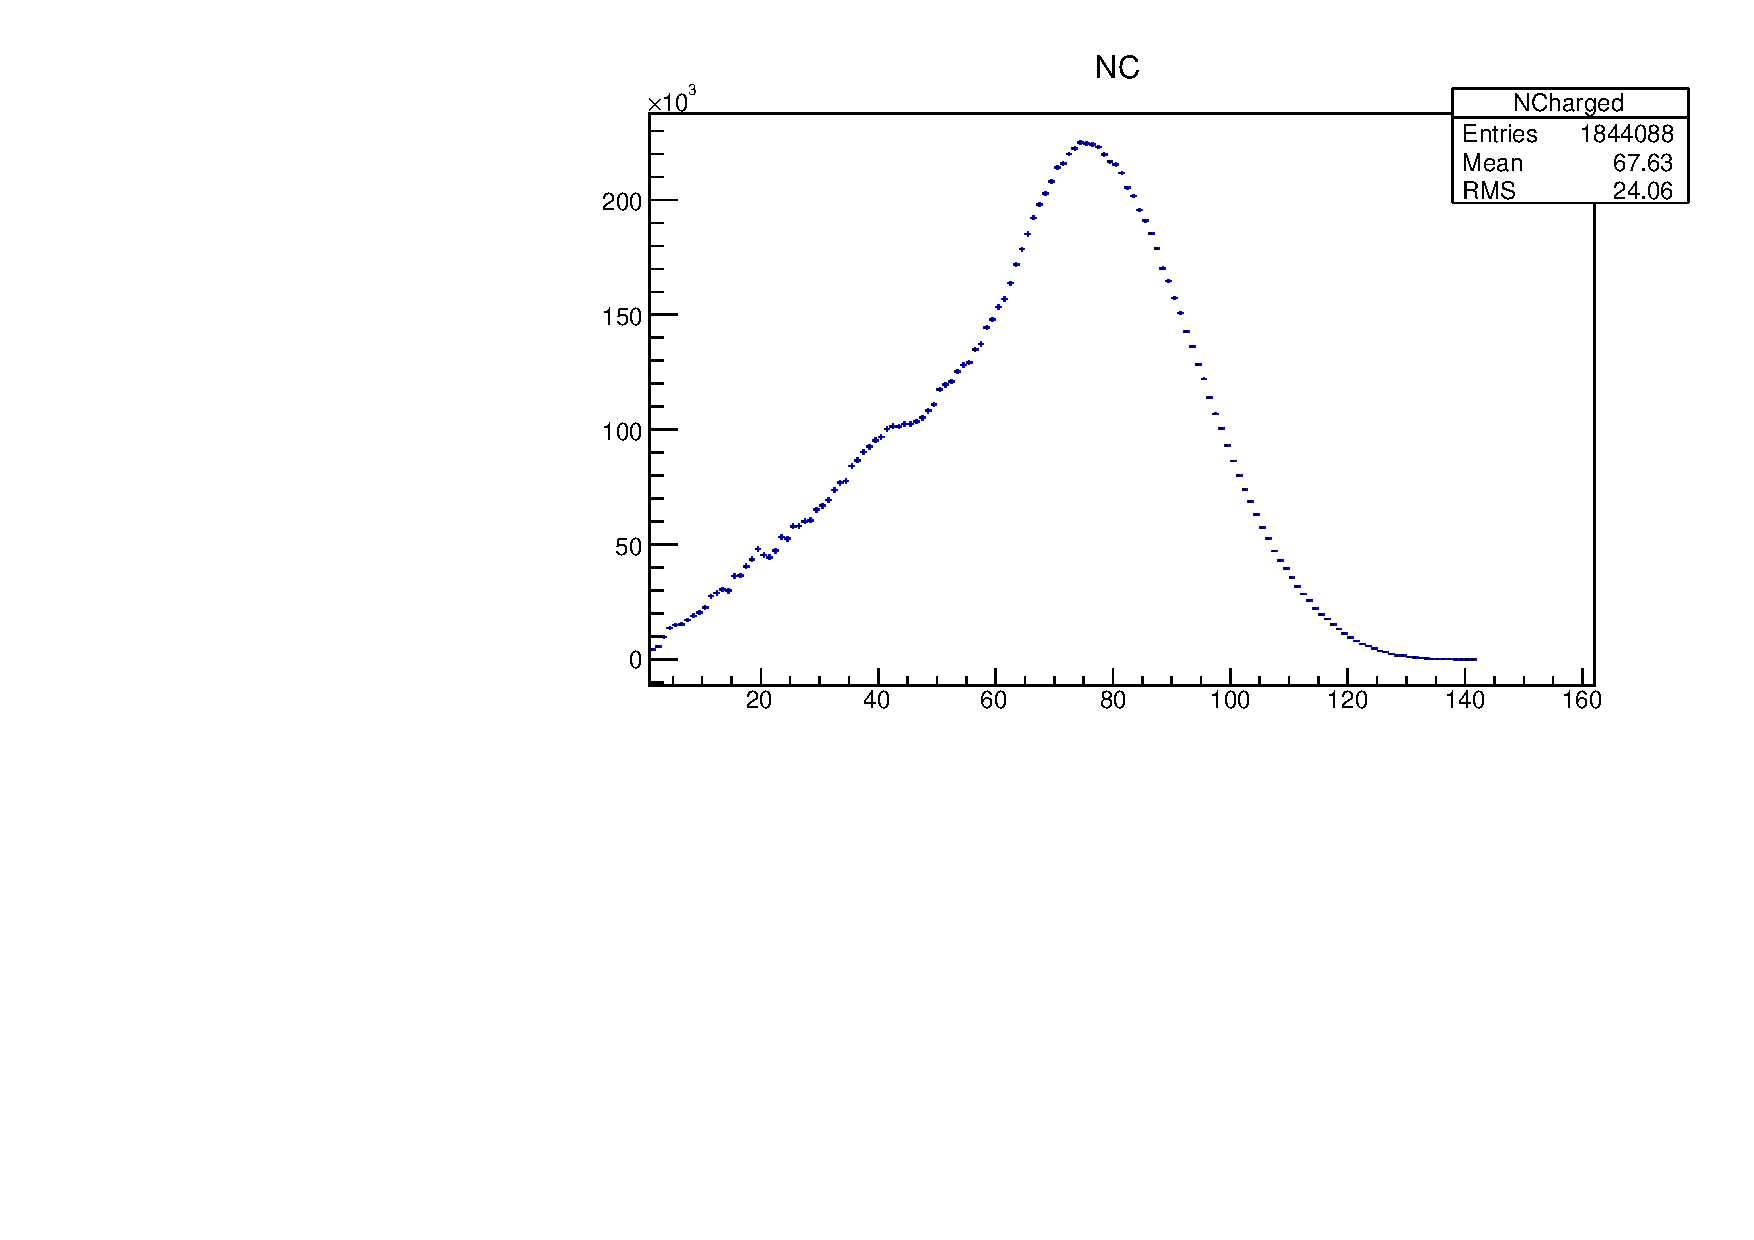
\includegraphics[width=\textwidth]{nc.pdf}
\caption{Number of detected charged particles in terms of kinetic energy of the missing particle after Carbon subtraction. }
\end{figure}

\begin{figure}
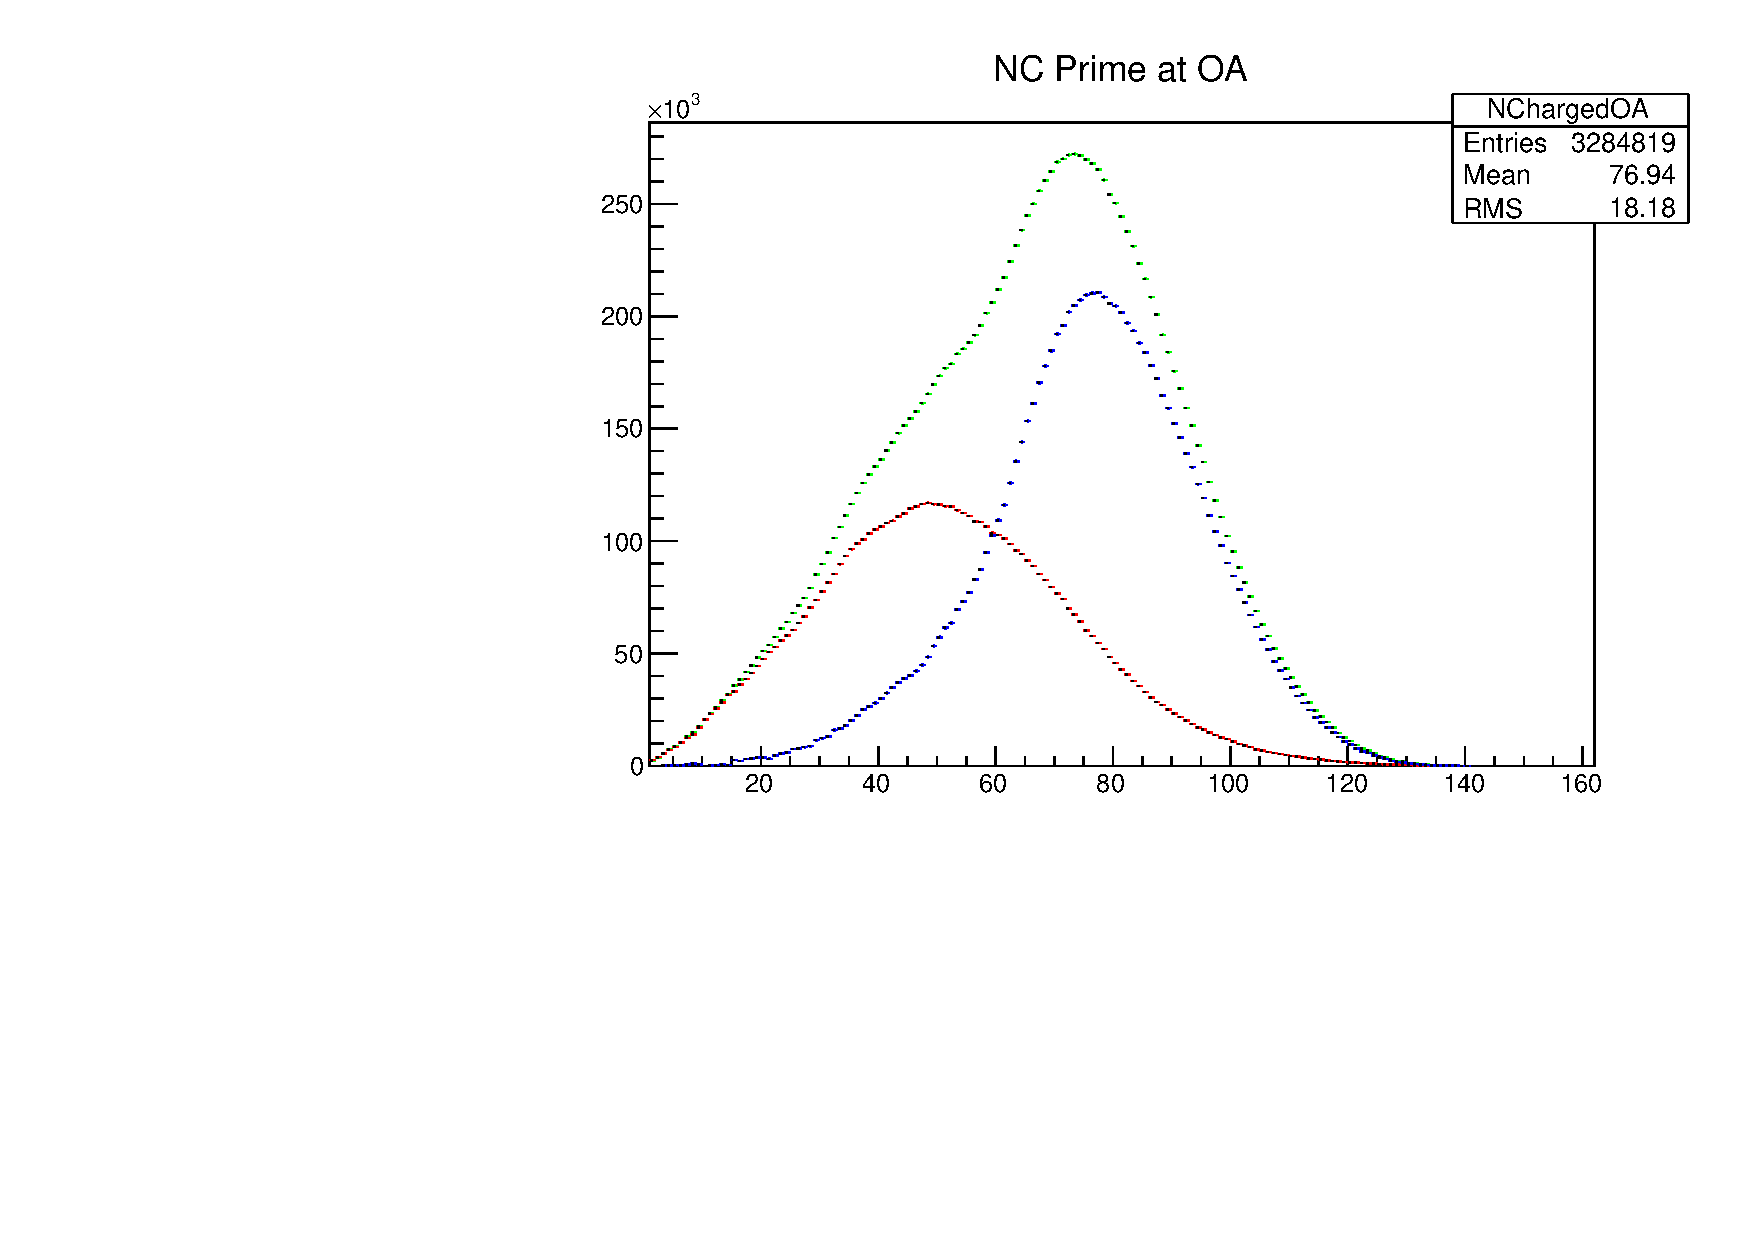
\includegraphics[width=\textwidth]{ncoa_b4.pdf}
\caption{Number of detected charged particles with in the opening angle cut, in terms of kinetic energy of the missing particle. }
\end{figure}

\begin{figure}
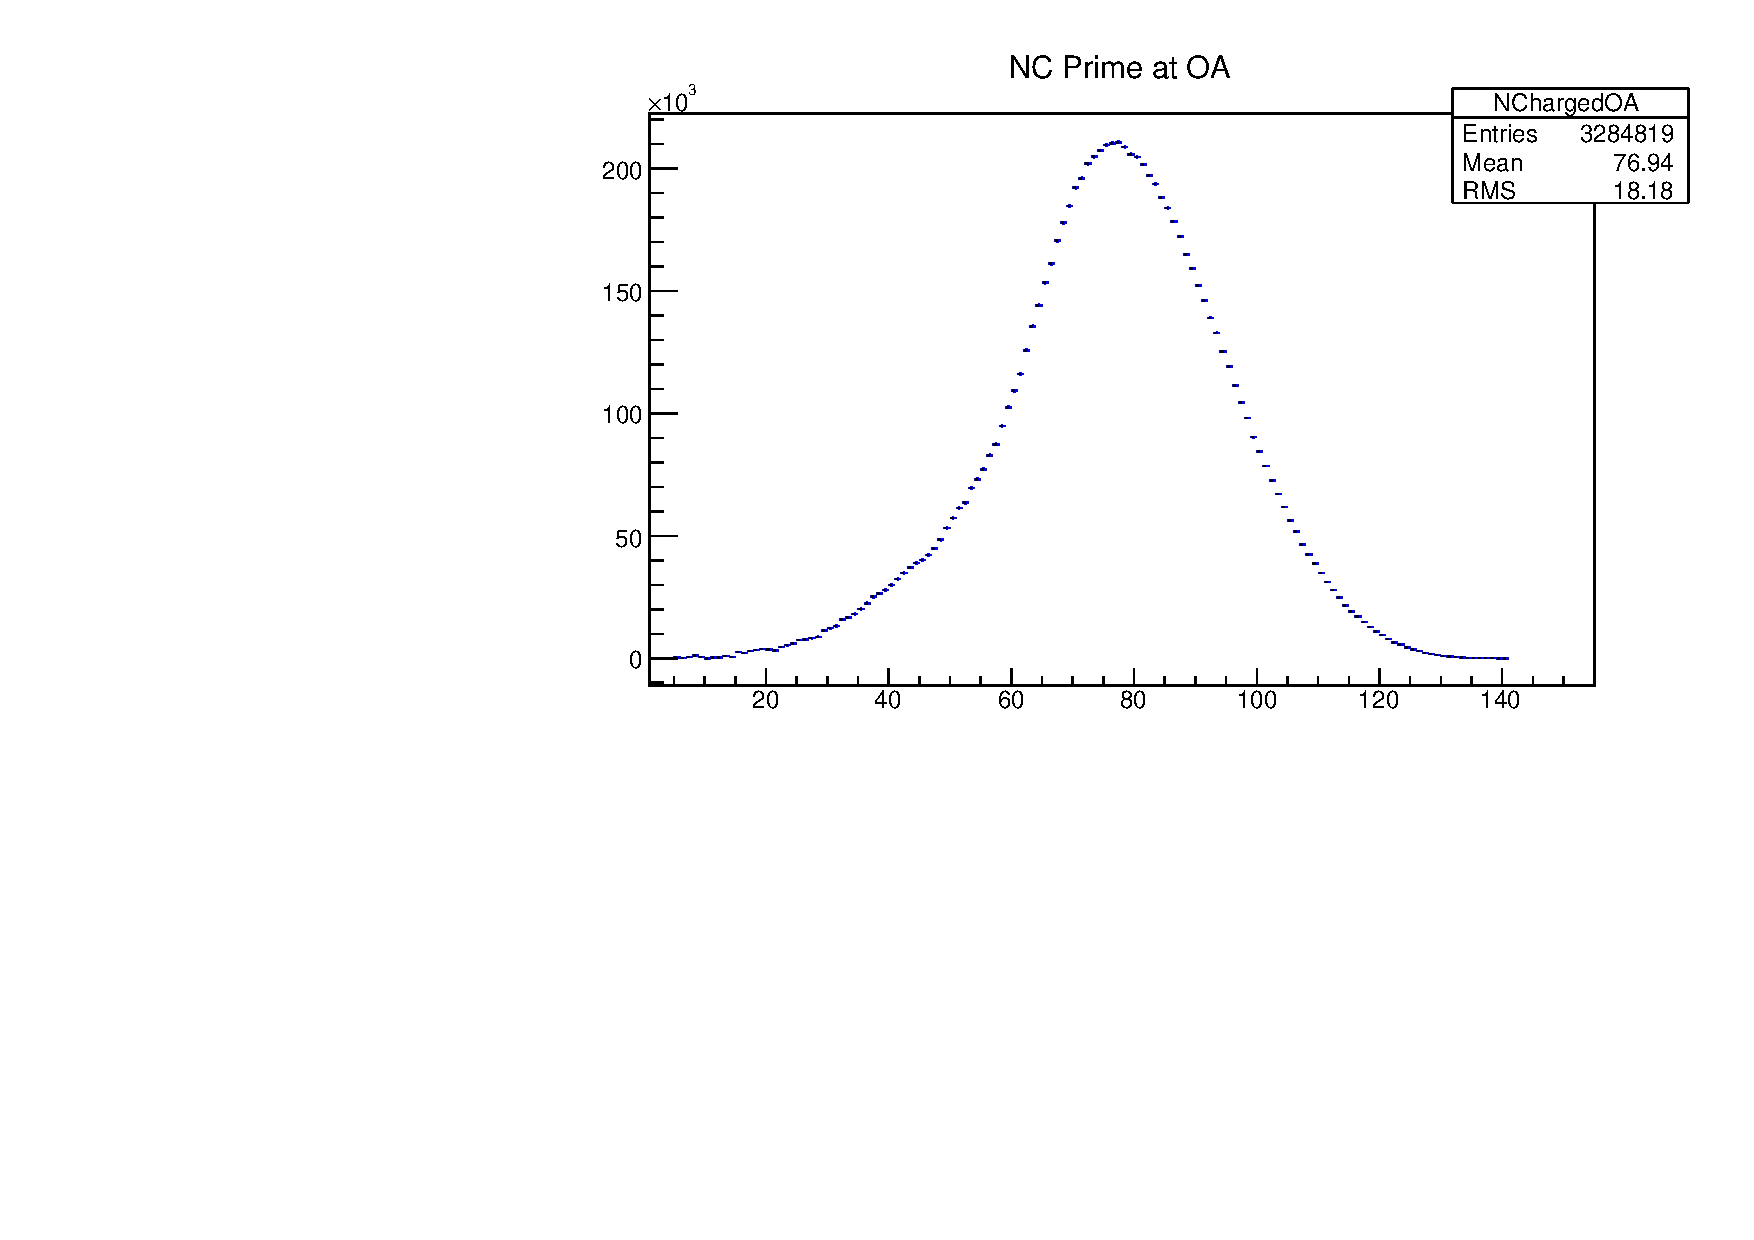
\includegraphics[width=\textwidth]{ncoa.pdf}
\caption{Number of detected charged particles with in the opening angle cut, in terms of kinetic energy of the missing particle after Carbon subtraction. }
\end{figure}

\begin{figure}
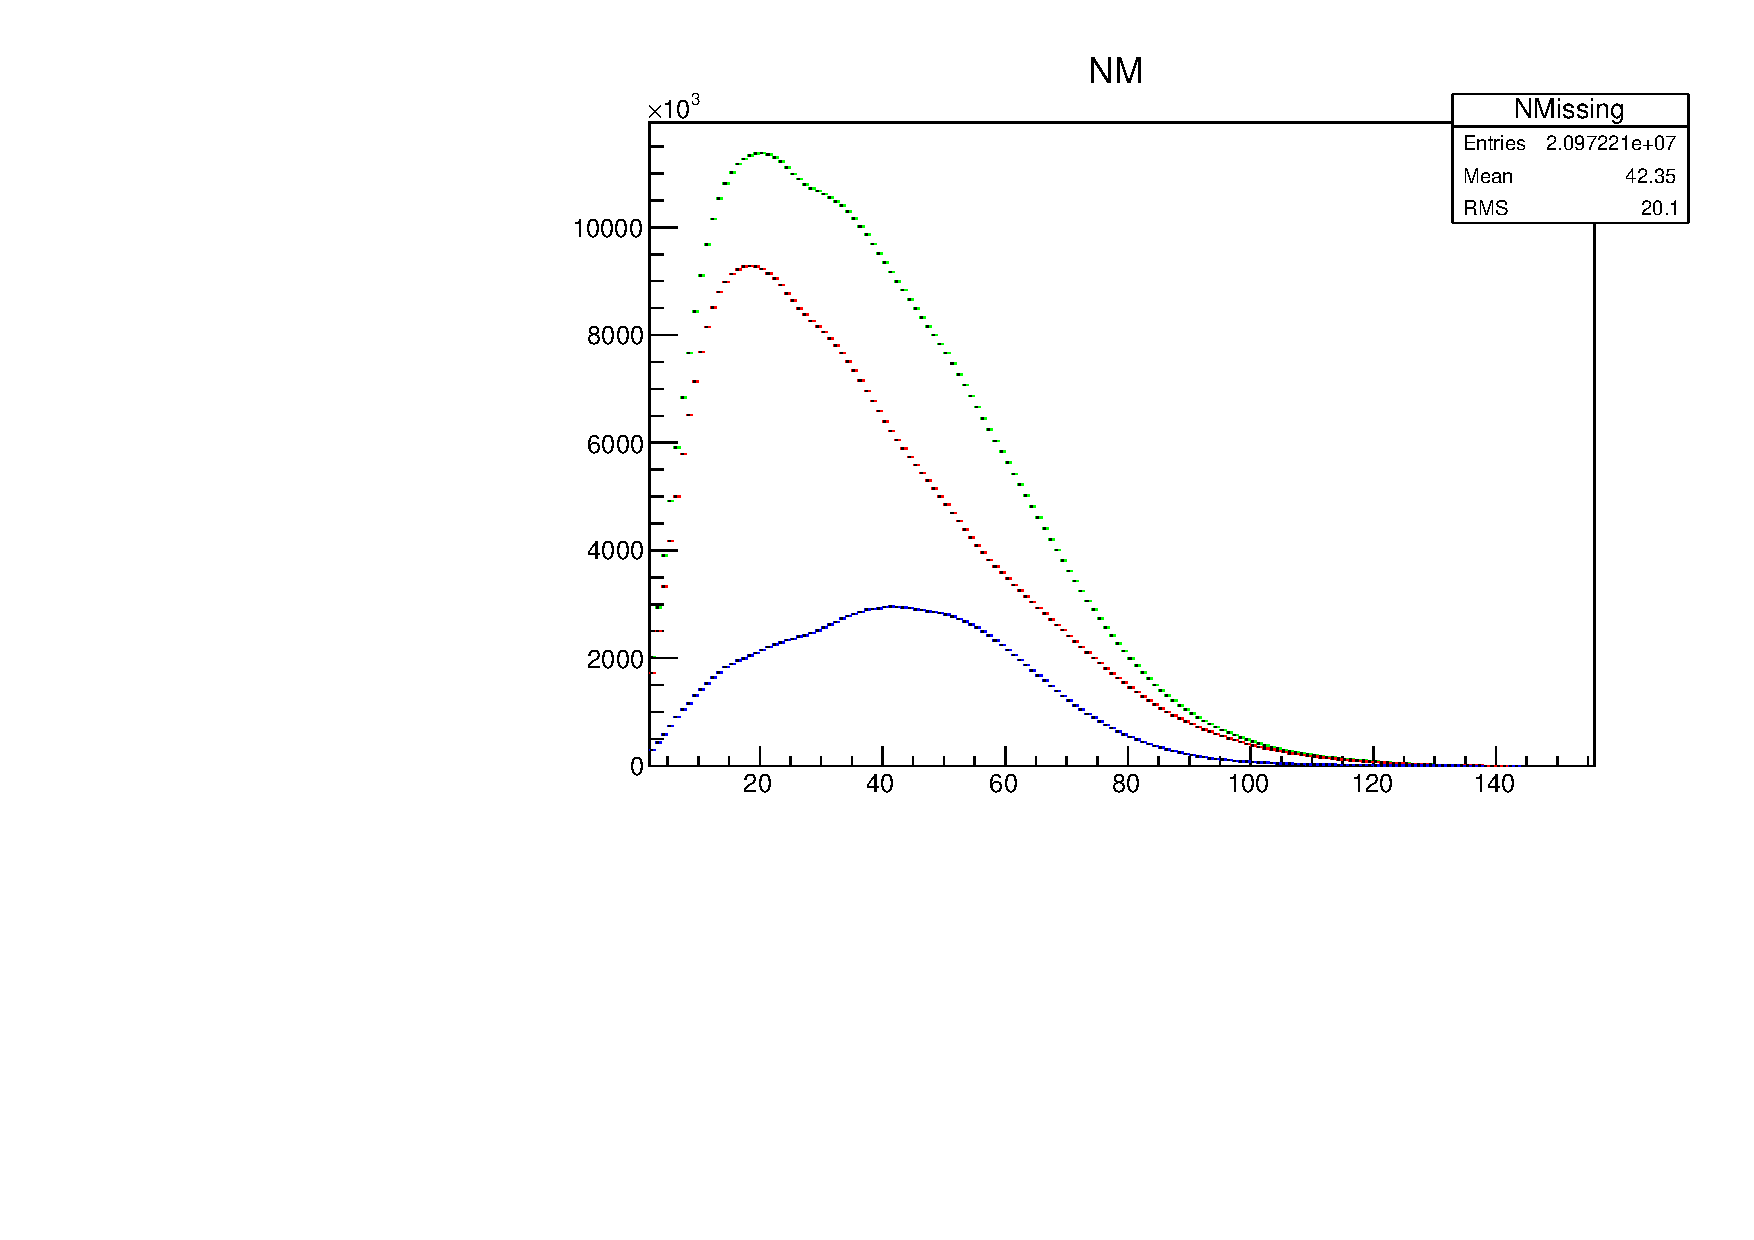
\includegraphics[width=\textwidth]{nm_b4.pdf}
\caption{Number of missing charged particles, in terms of kinetic energy of the missing particle. }
\end{figure}

\begin{figure}
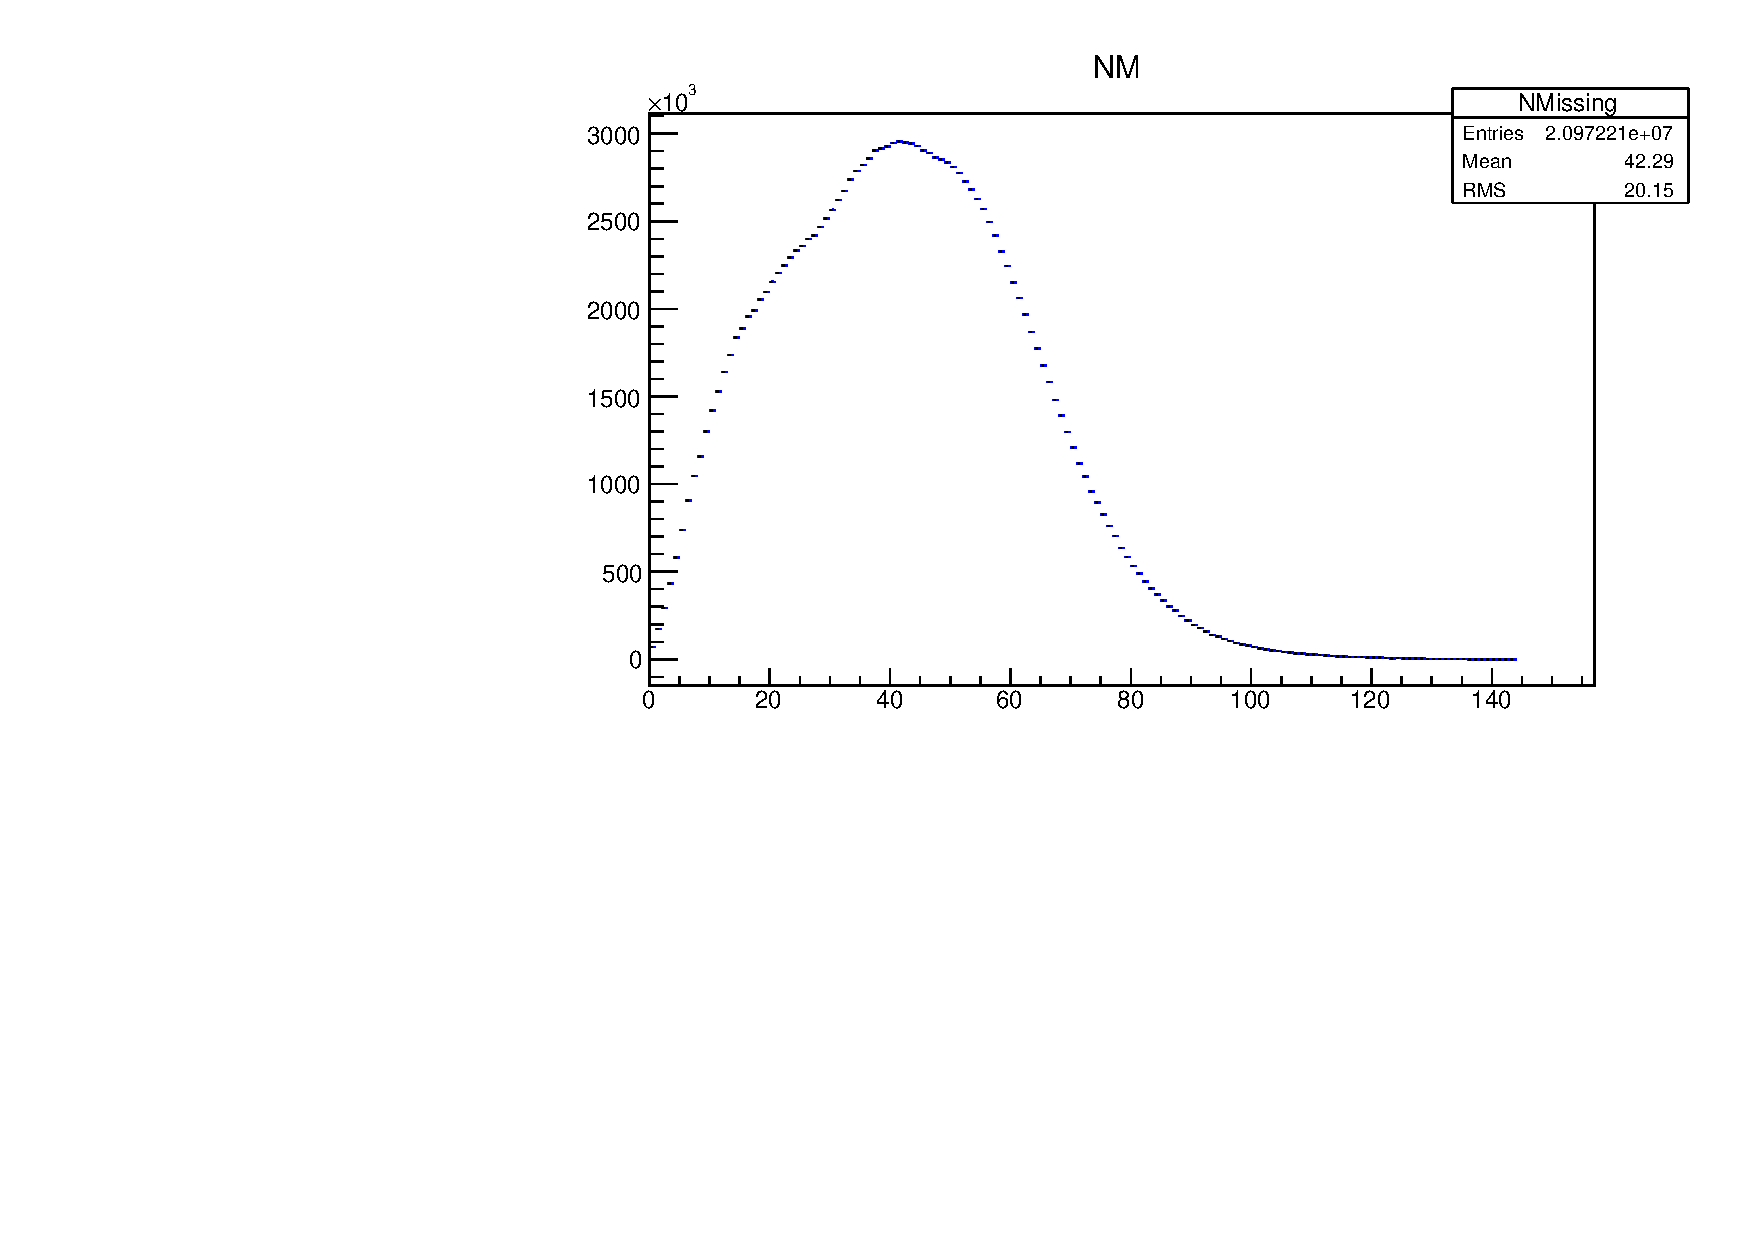
\includegraphics[width=\textwidth]{nm.pdf}
\caption{Number of missing charged particles, in terms of kinetic energy of the missing particle after Carbon subtraction. }
\end{figure}

\begin{figure}
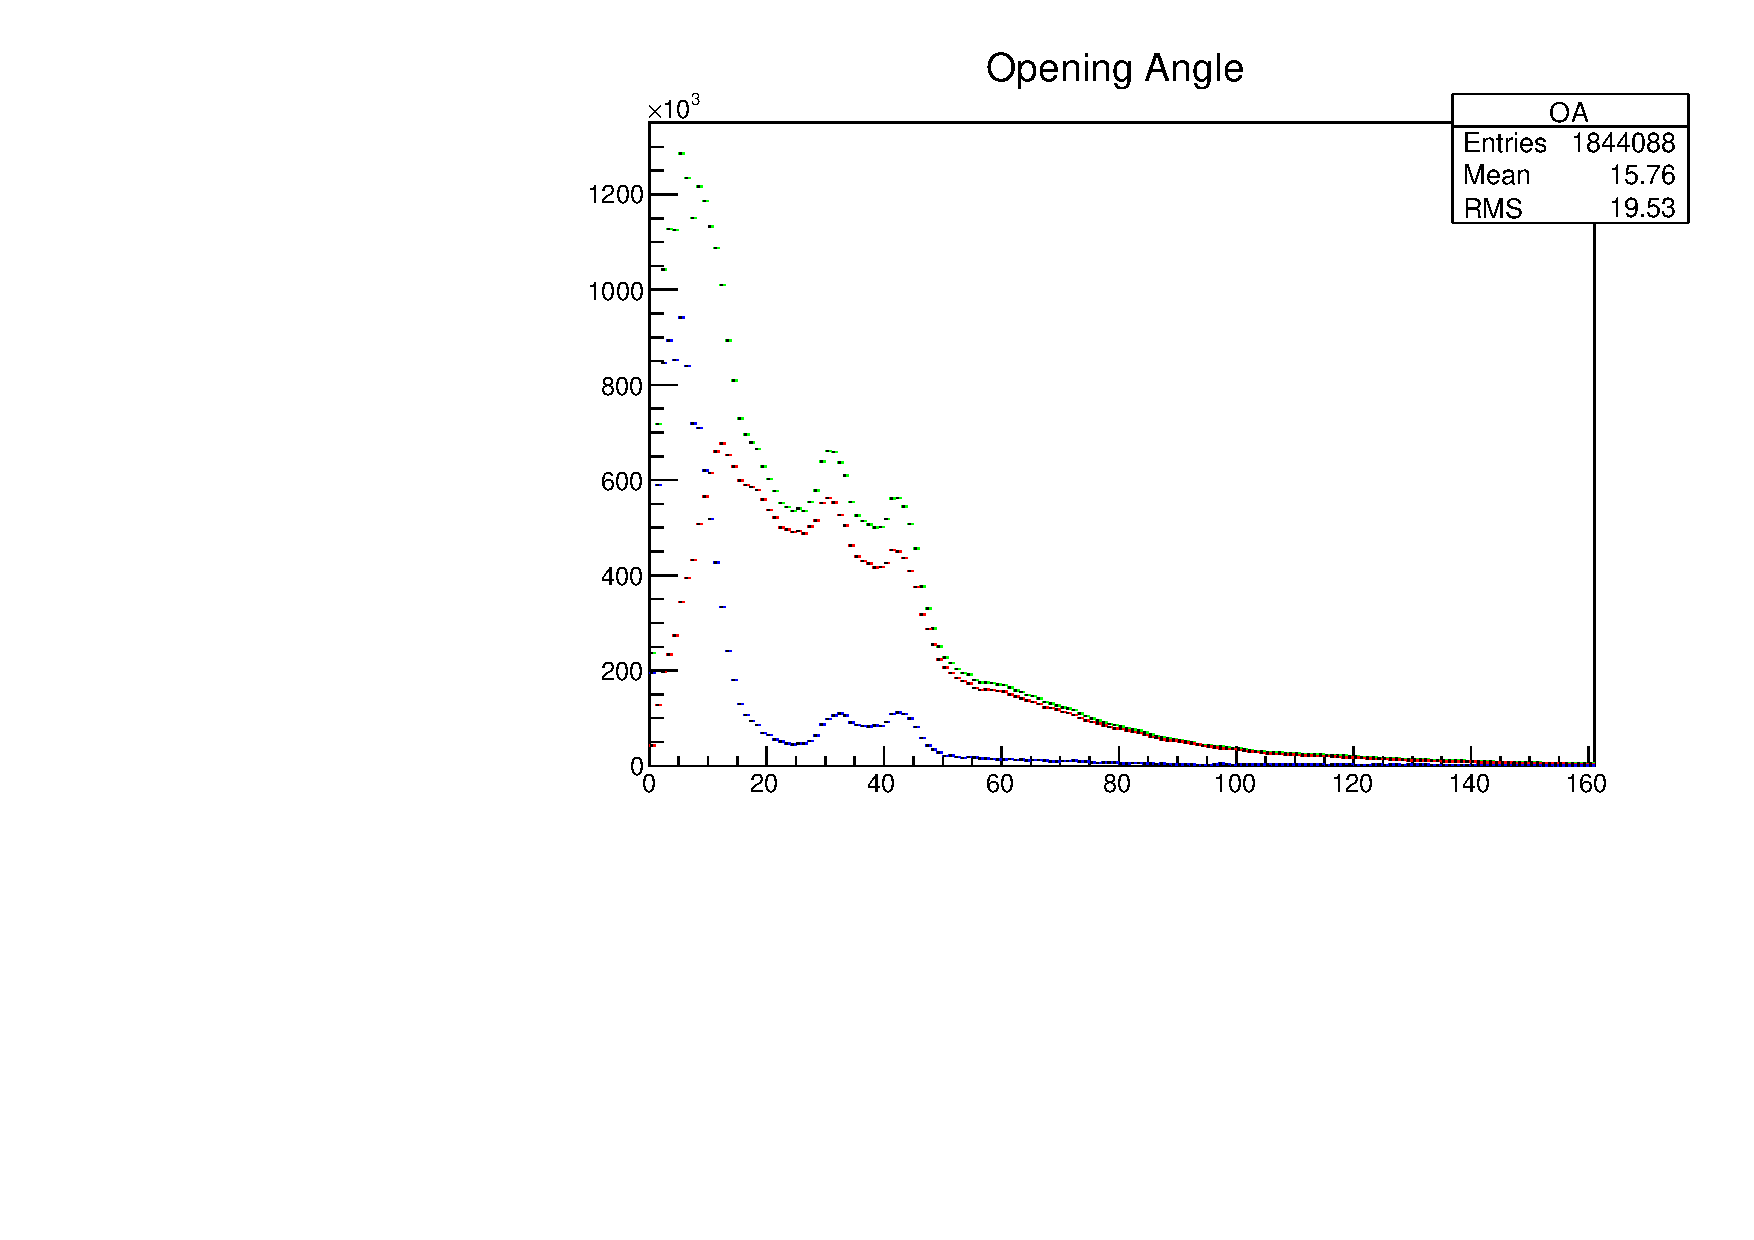
\includegraphics[width=\textwidth]{oa_b4.pdf}
\caption{Opening angle distribution, in terms of kinetic energy of the missing particle.Green being Butanol data, Red Carbon and Blue subtracted distribution. }
\end{figure}

\begin{figure}
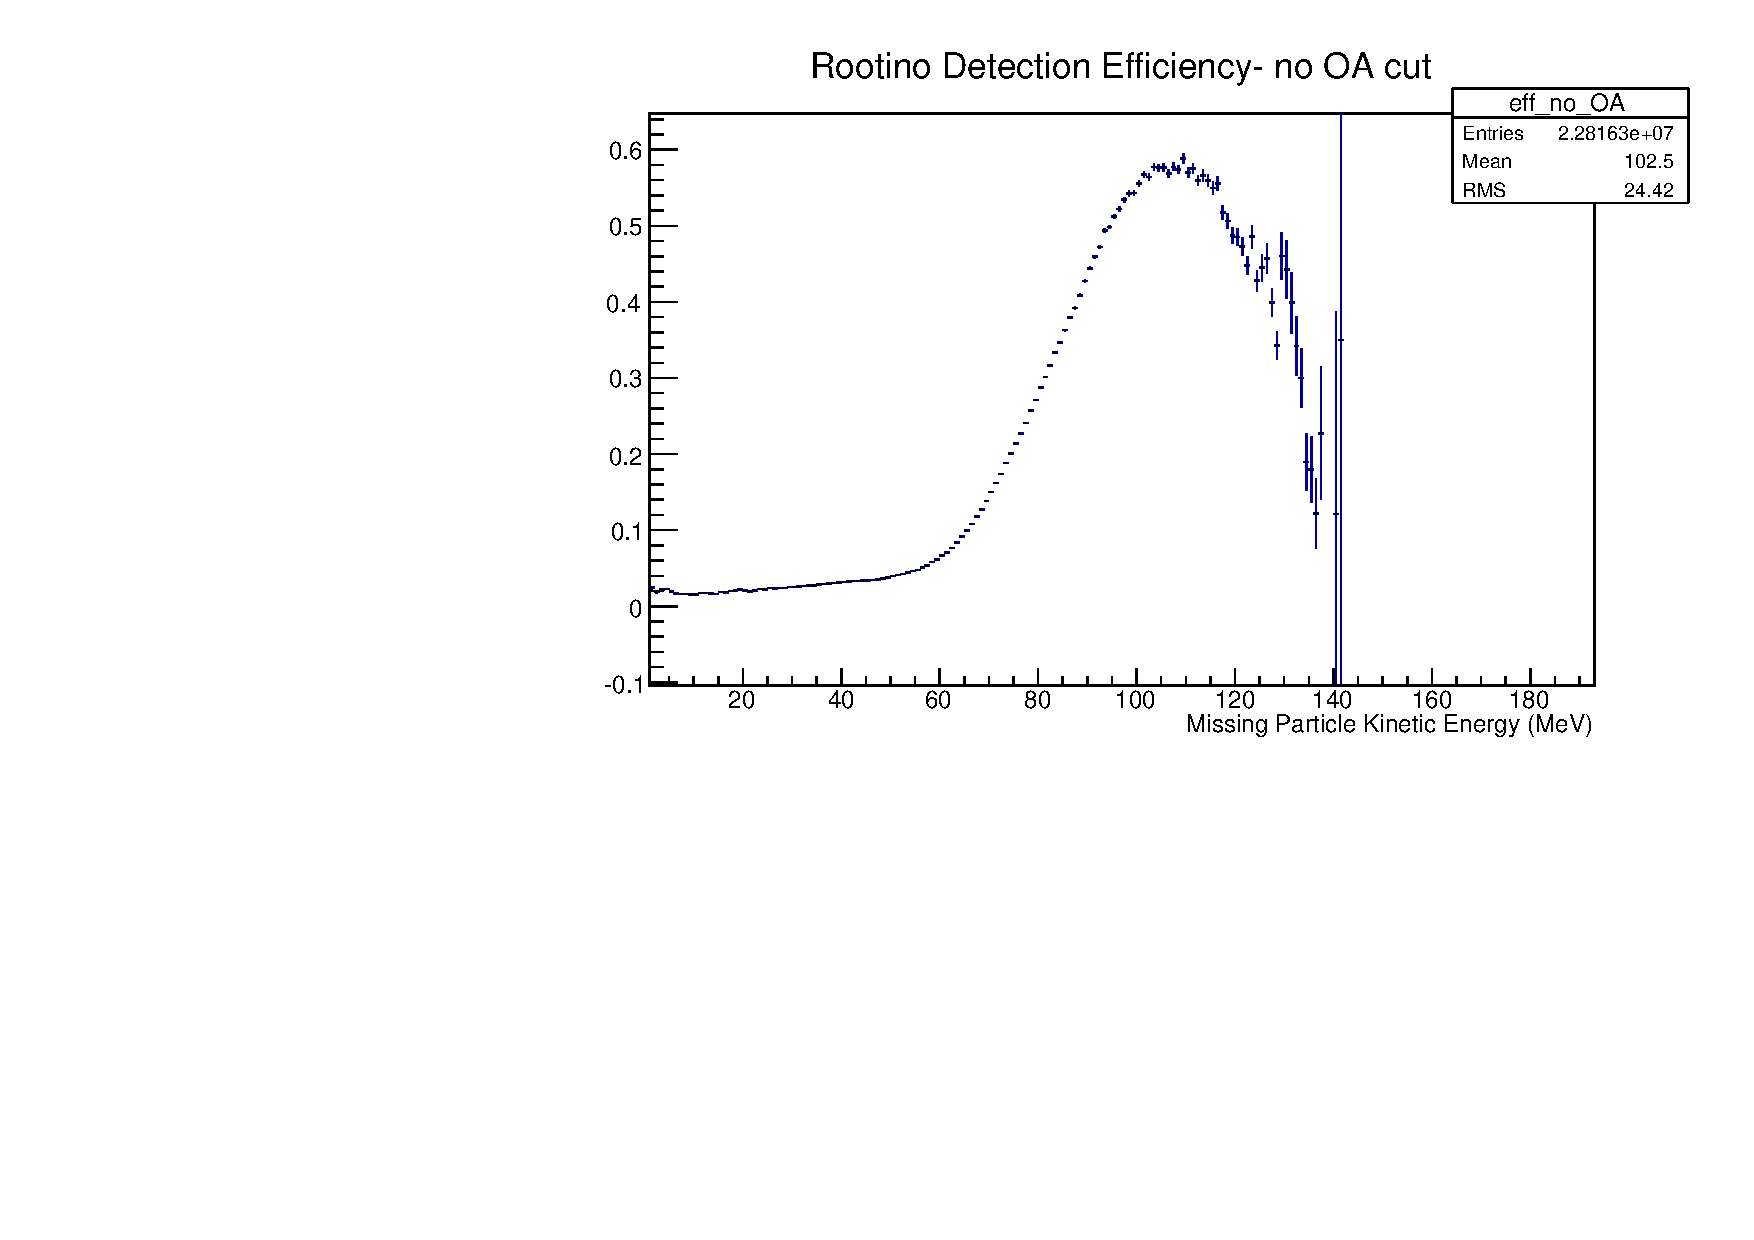
\includegraphics[width=\textwidth]{eff_no_oa.pdf}
\caption{Rootino detection efficiency, with no opening angle cut applied. }
\end{figure}

\begin{figure}
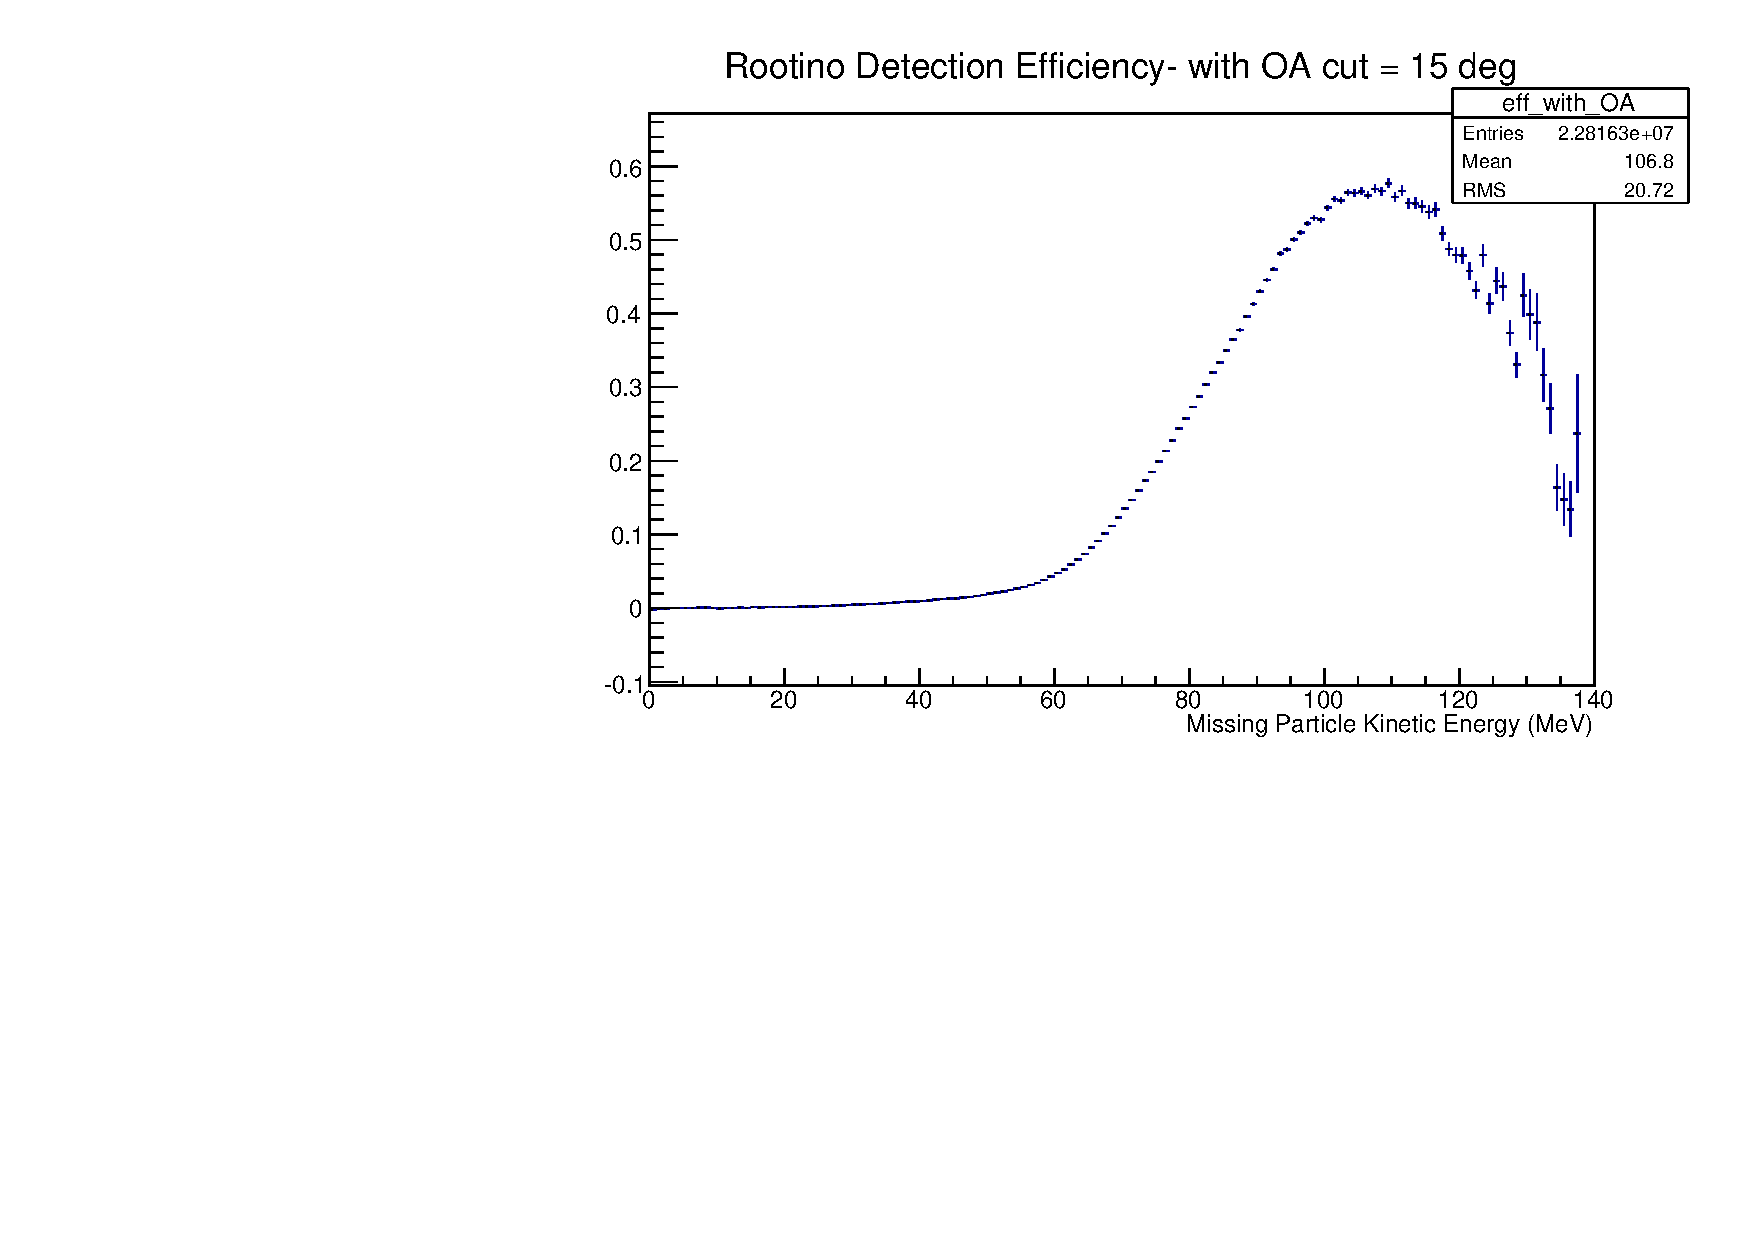
\includegraphics[width=\textwidth]{eff_oa.pdf}
\caption{Rootino detection efficiency, with opening angle cut = $15^{\circ}$  }
\end{figure}

\begin{figure}
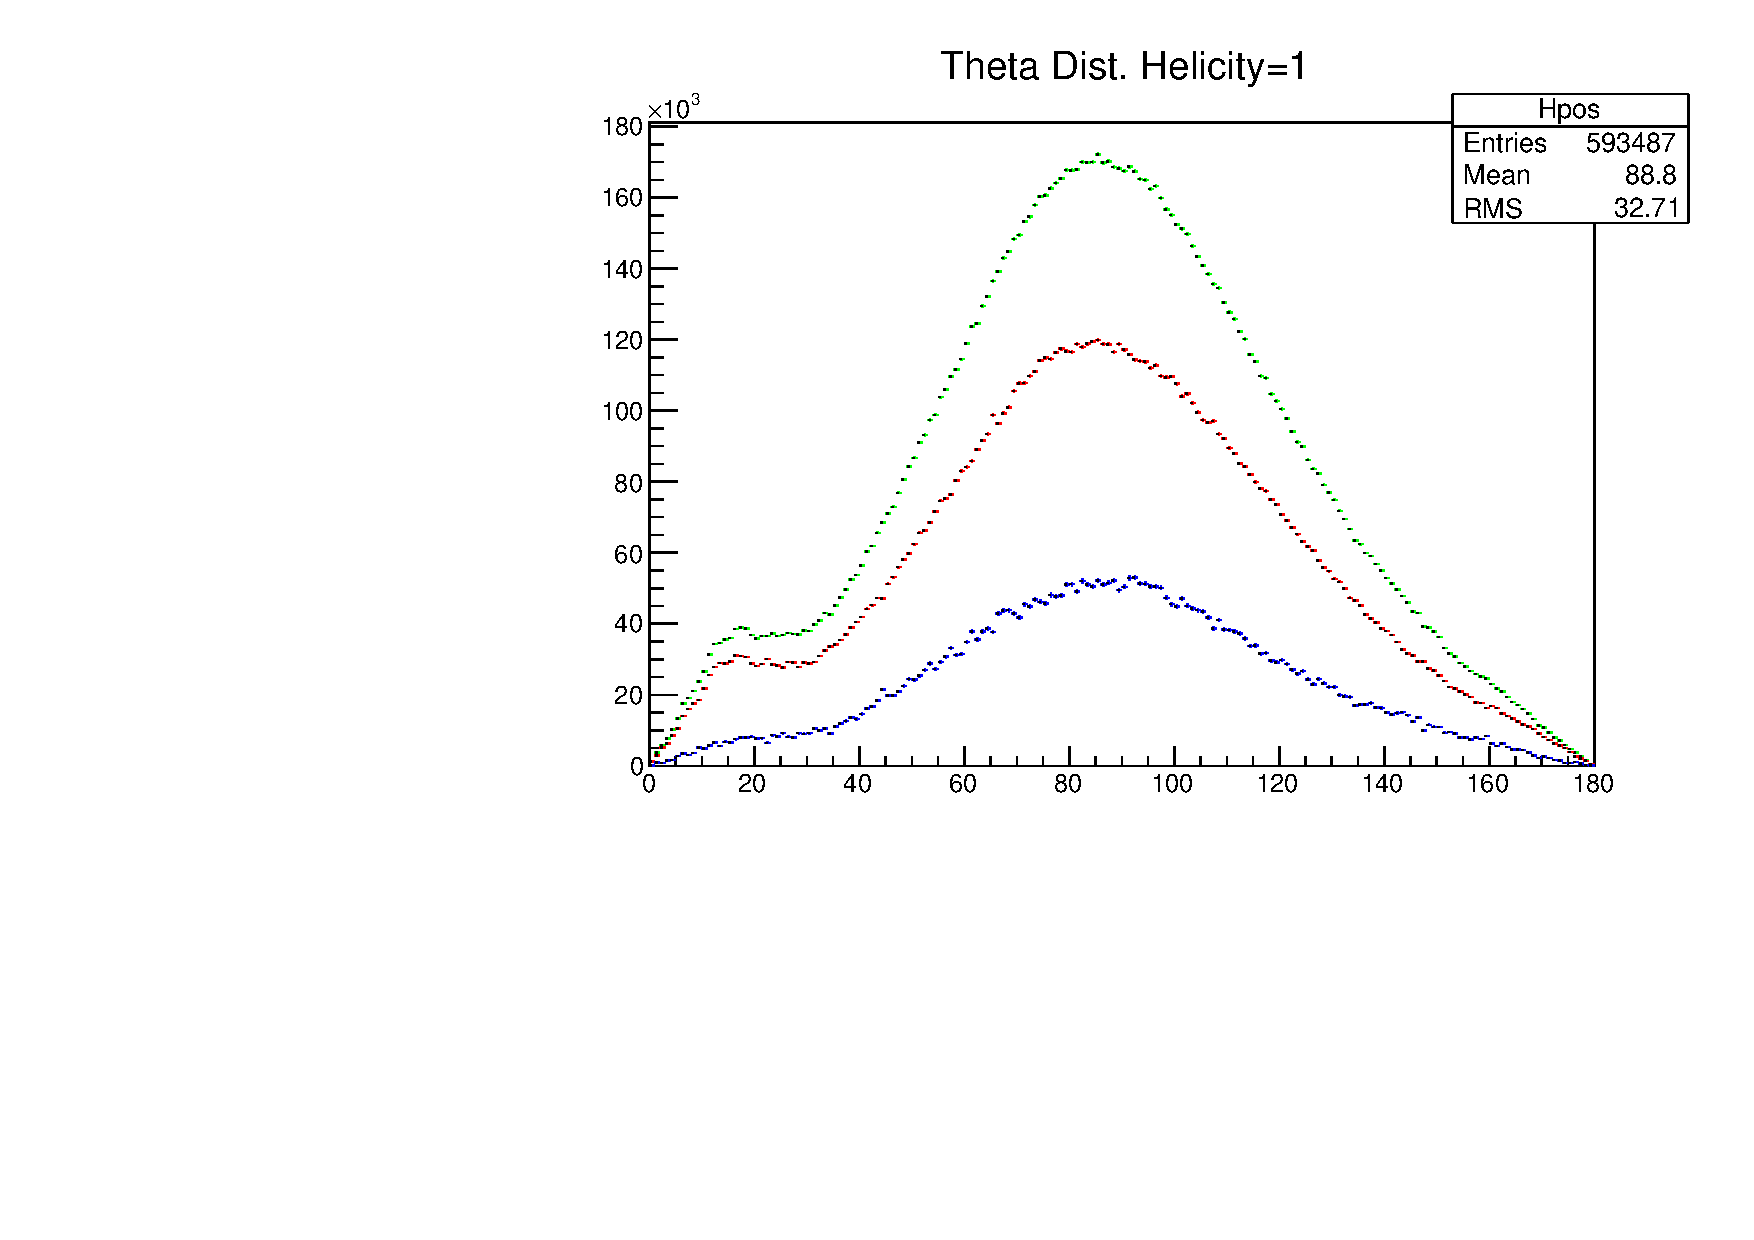
\includegraphics[width=\textwidth]{Asym/Theta_h1_b4.pdf}
\caption{Theta distribution for events with helicity = +1, butanol (green), carbon (red) and subtracted (blue). }
\end{figure}

\begin{figure}
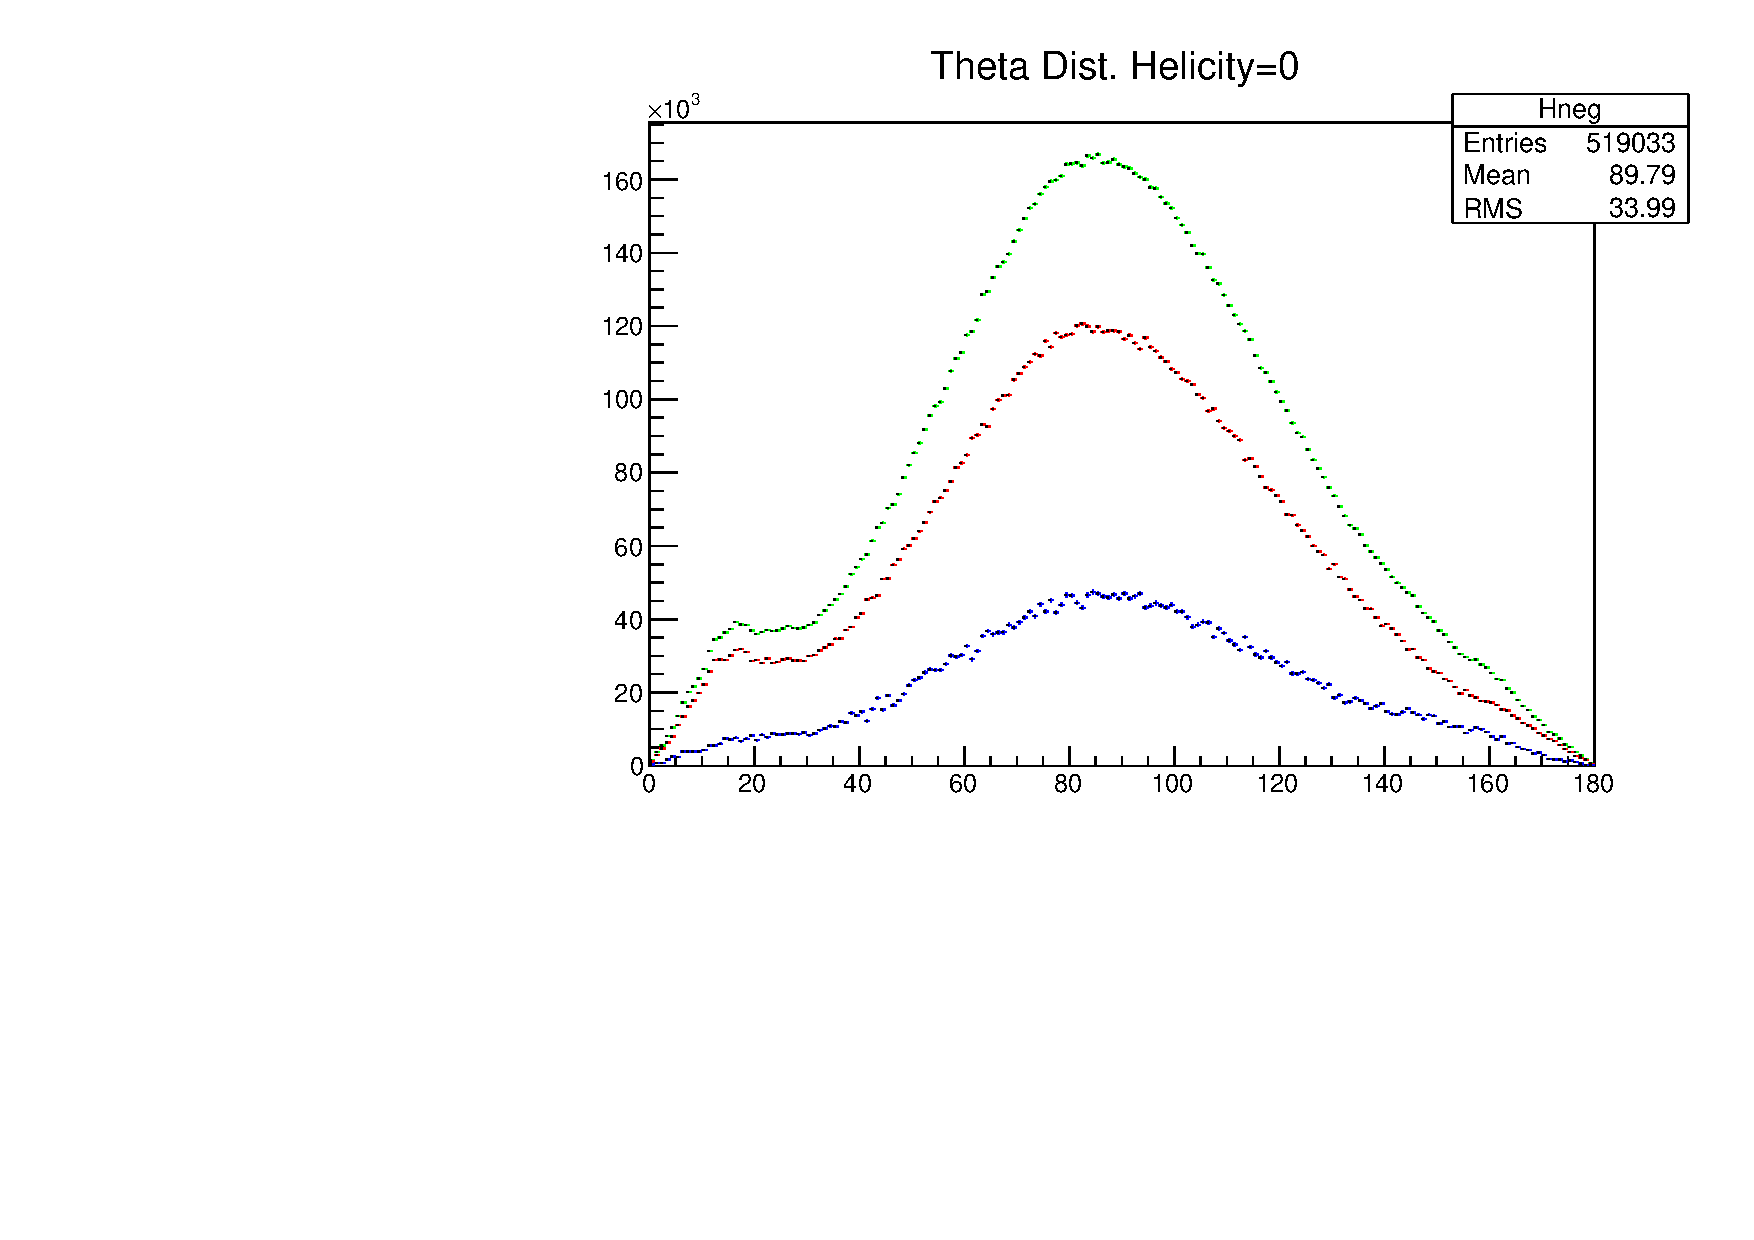
\includegraphics[width=\textwidth]{Asym/Theta_h0_b4.pdf}
\caption{Theta distribution for events with helicity = 0, butanol (green), carbon (red) and subtracted (blue). }
\end{figure}

\begin{figure}
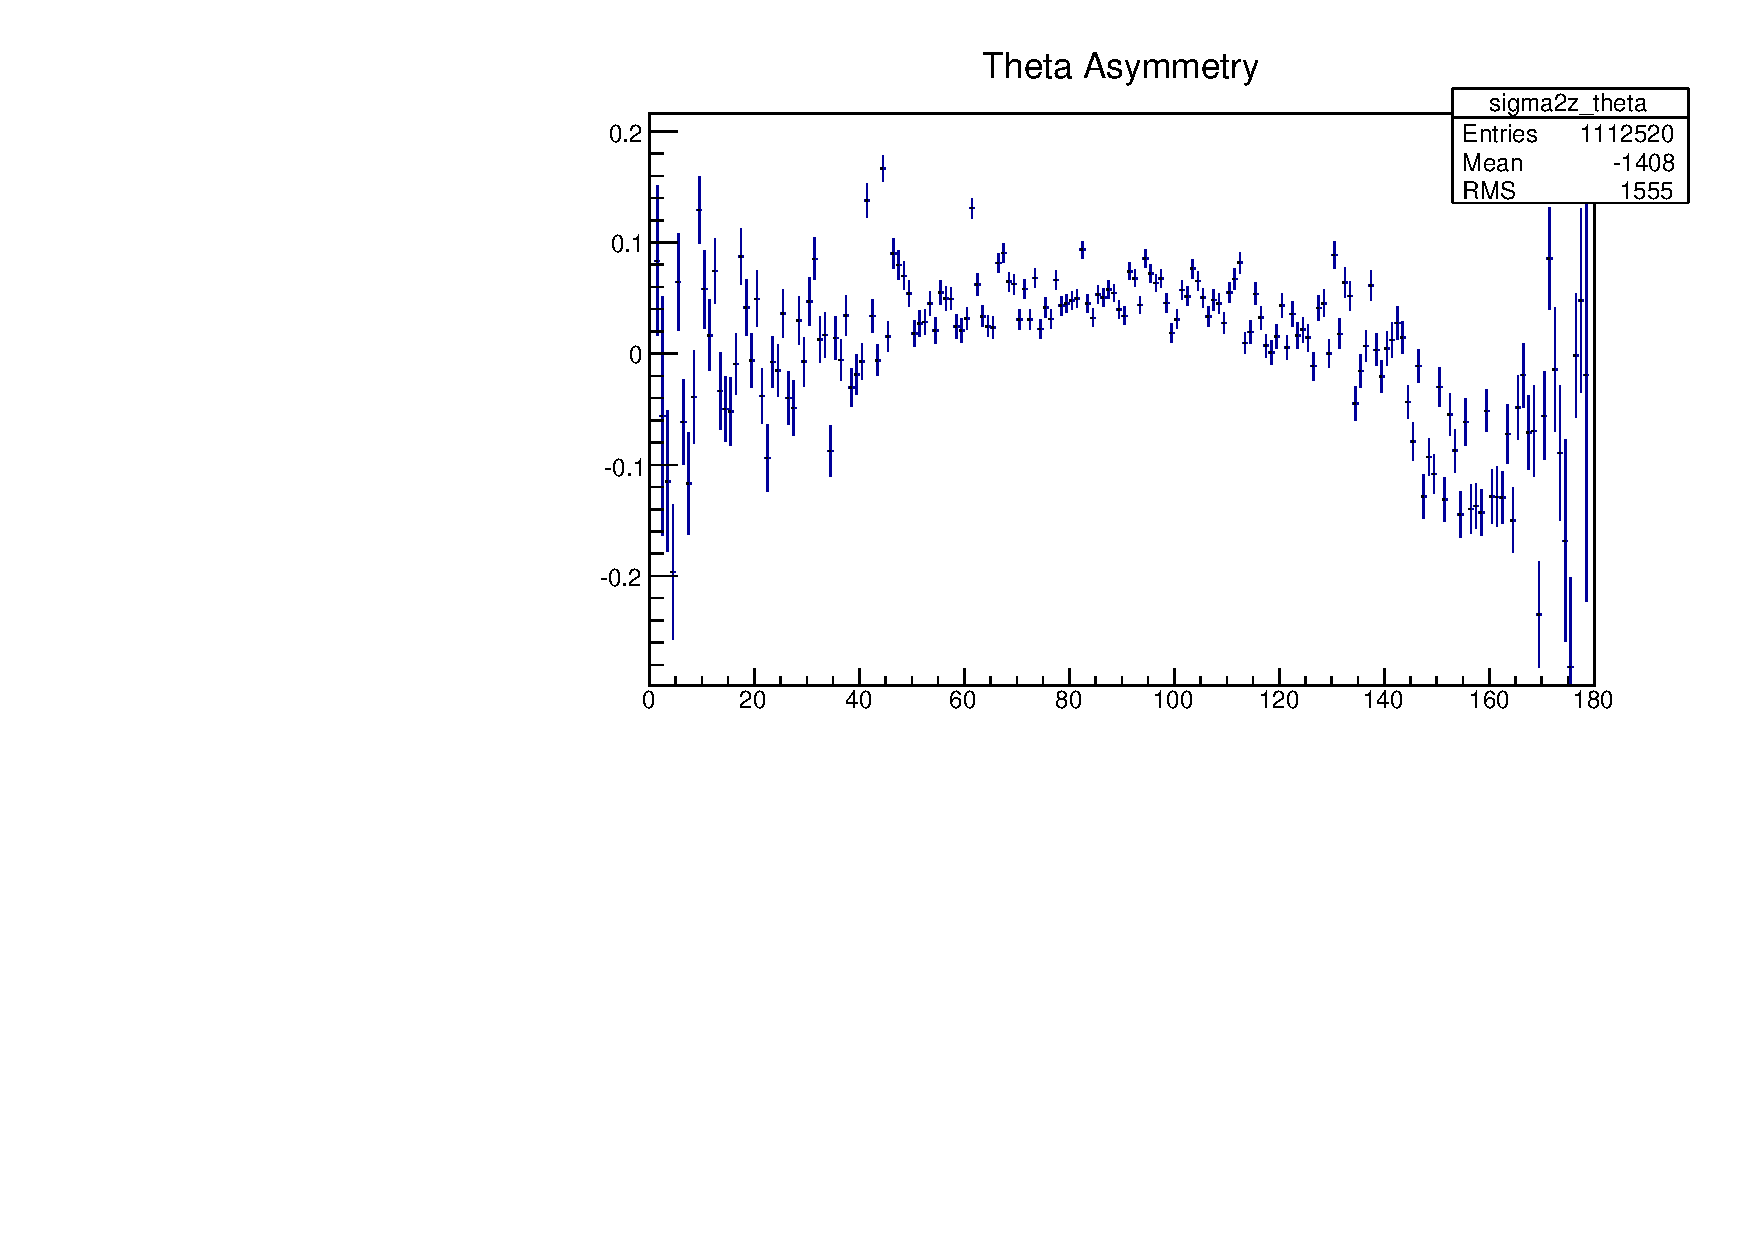
\includegraphics[width=\textwidth]{Asym/theta_asym.pdf}
\caption{Theta asymmetry with no angle cut. }
\end{figure}

\begin{figure}
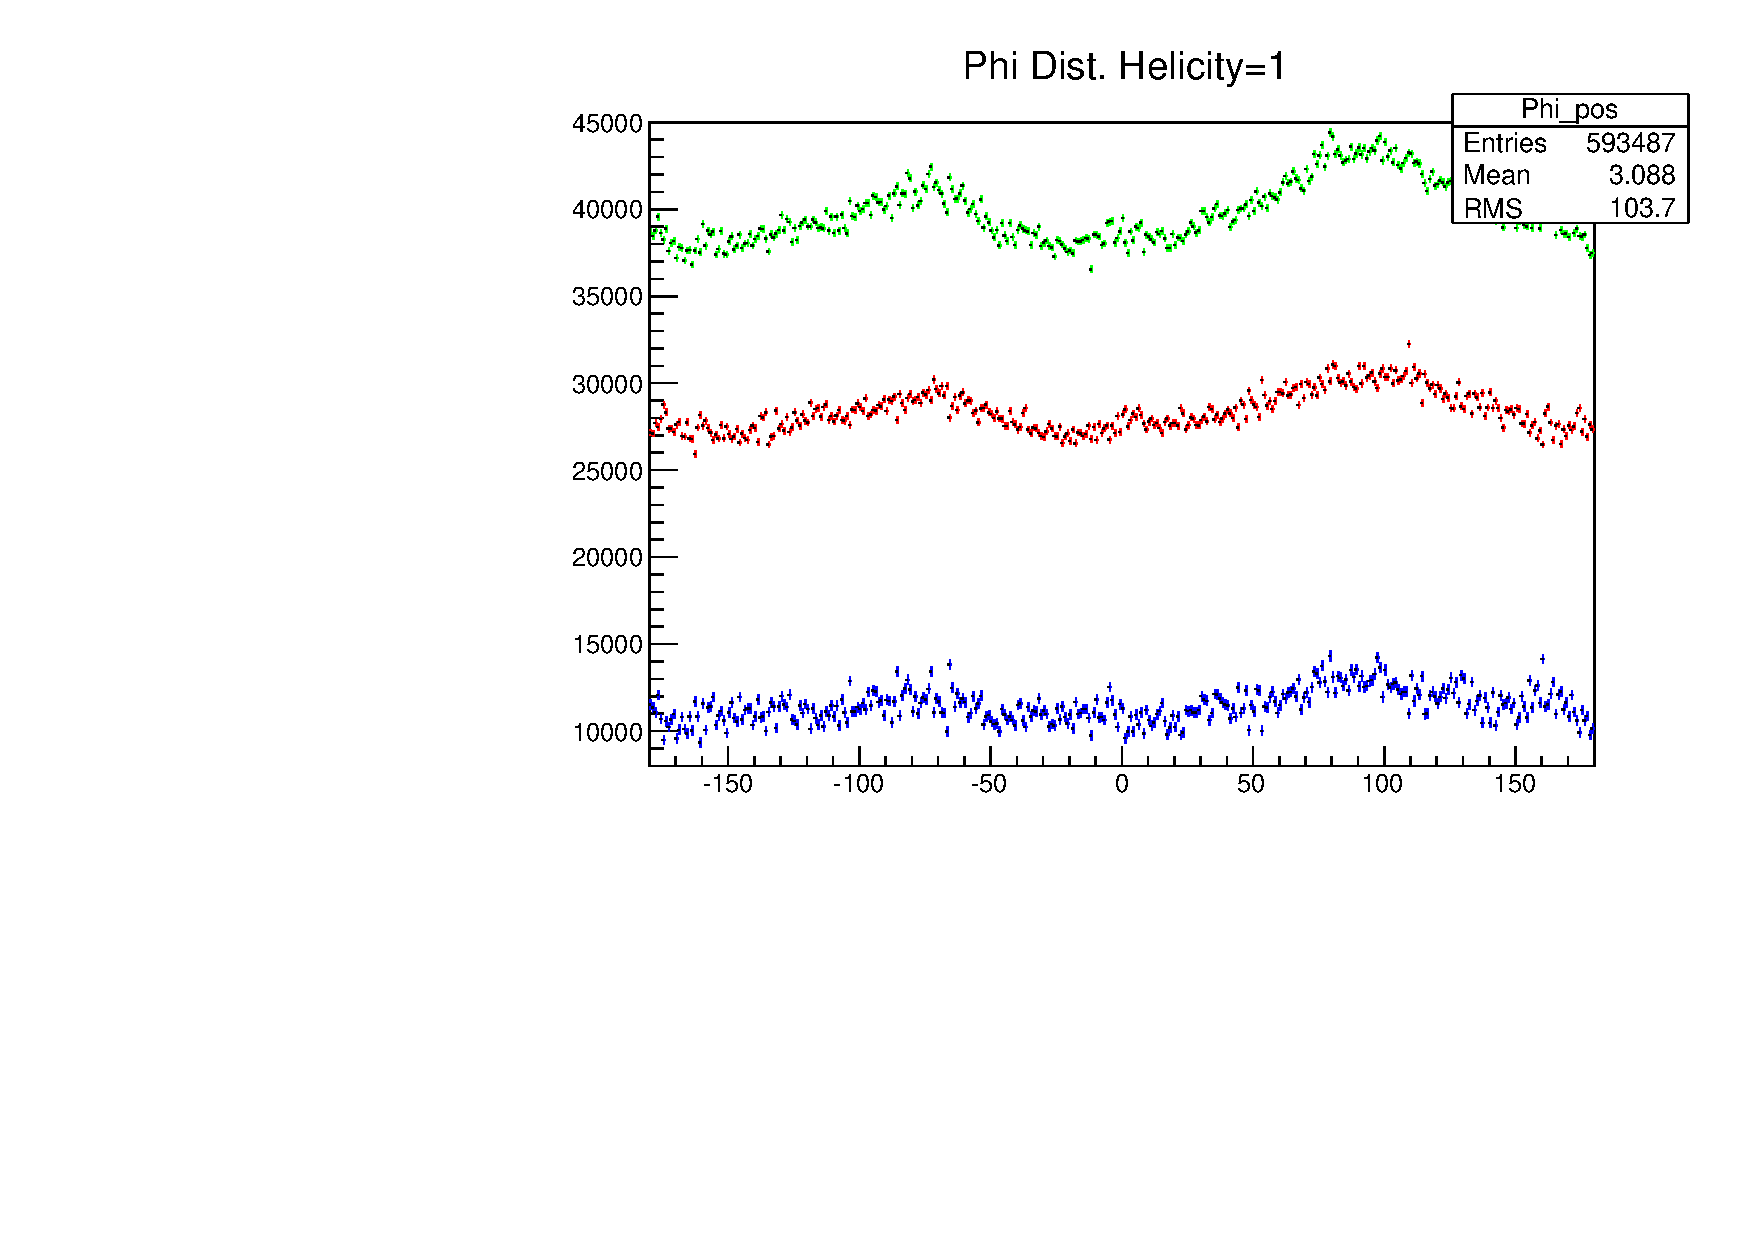
\includegraphics[width=\textwidth]{Asym/Phi_h1_b4.pdf}
\caption{Phi distribution for events with helicity = +1, butanol (green), carbon (red) and subtracted (blue). }
\end{figure}

\begin{figure}
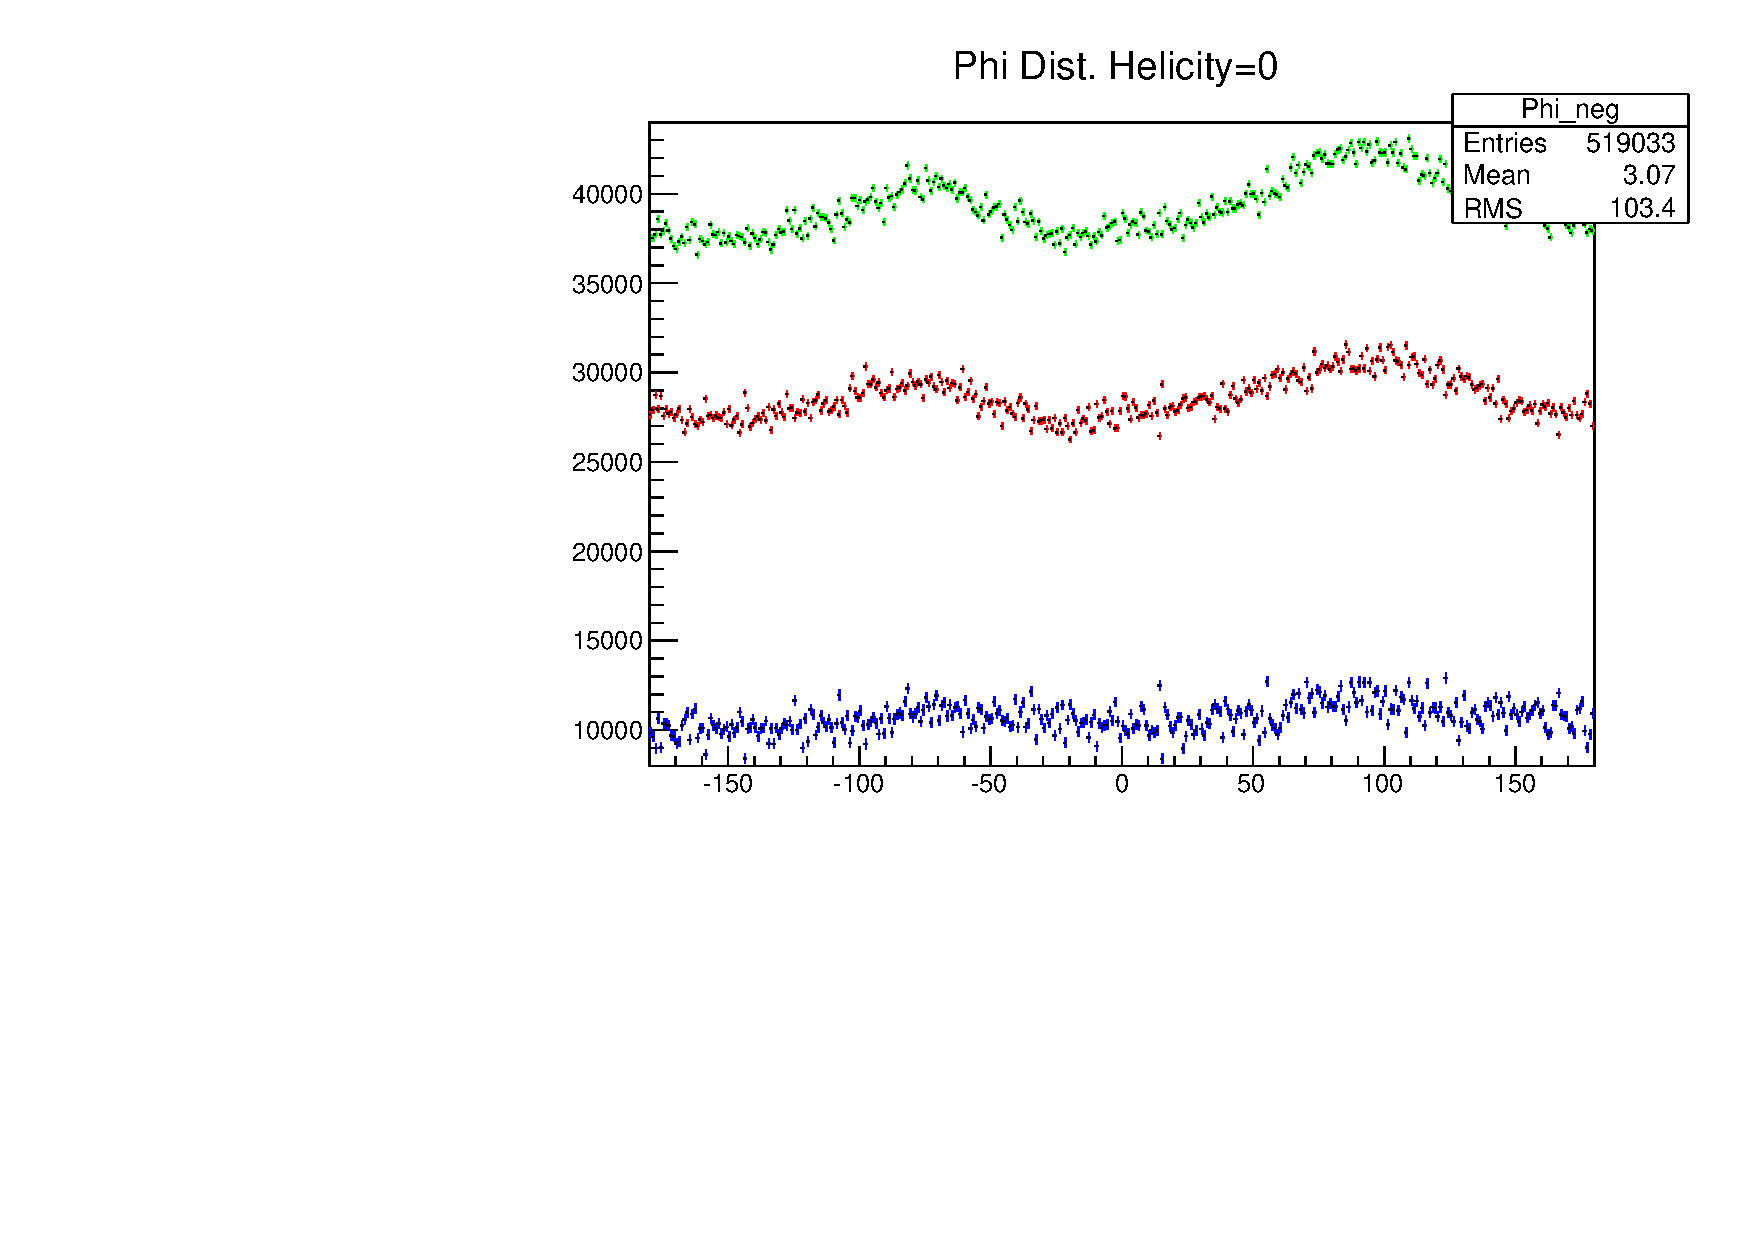
\includegraphics[width=\textwidth]{Asym/Phi_h0_b4.pdf}
\caption{Phi distribution for events with helicity = 0, butanol (green), carbon (red) and subtracted (blue). }
\end{figure}

\begin{figure}
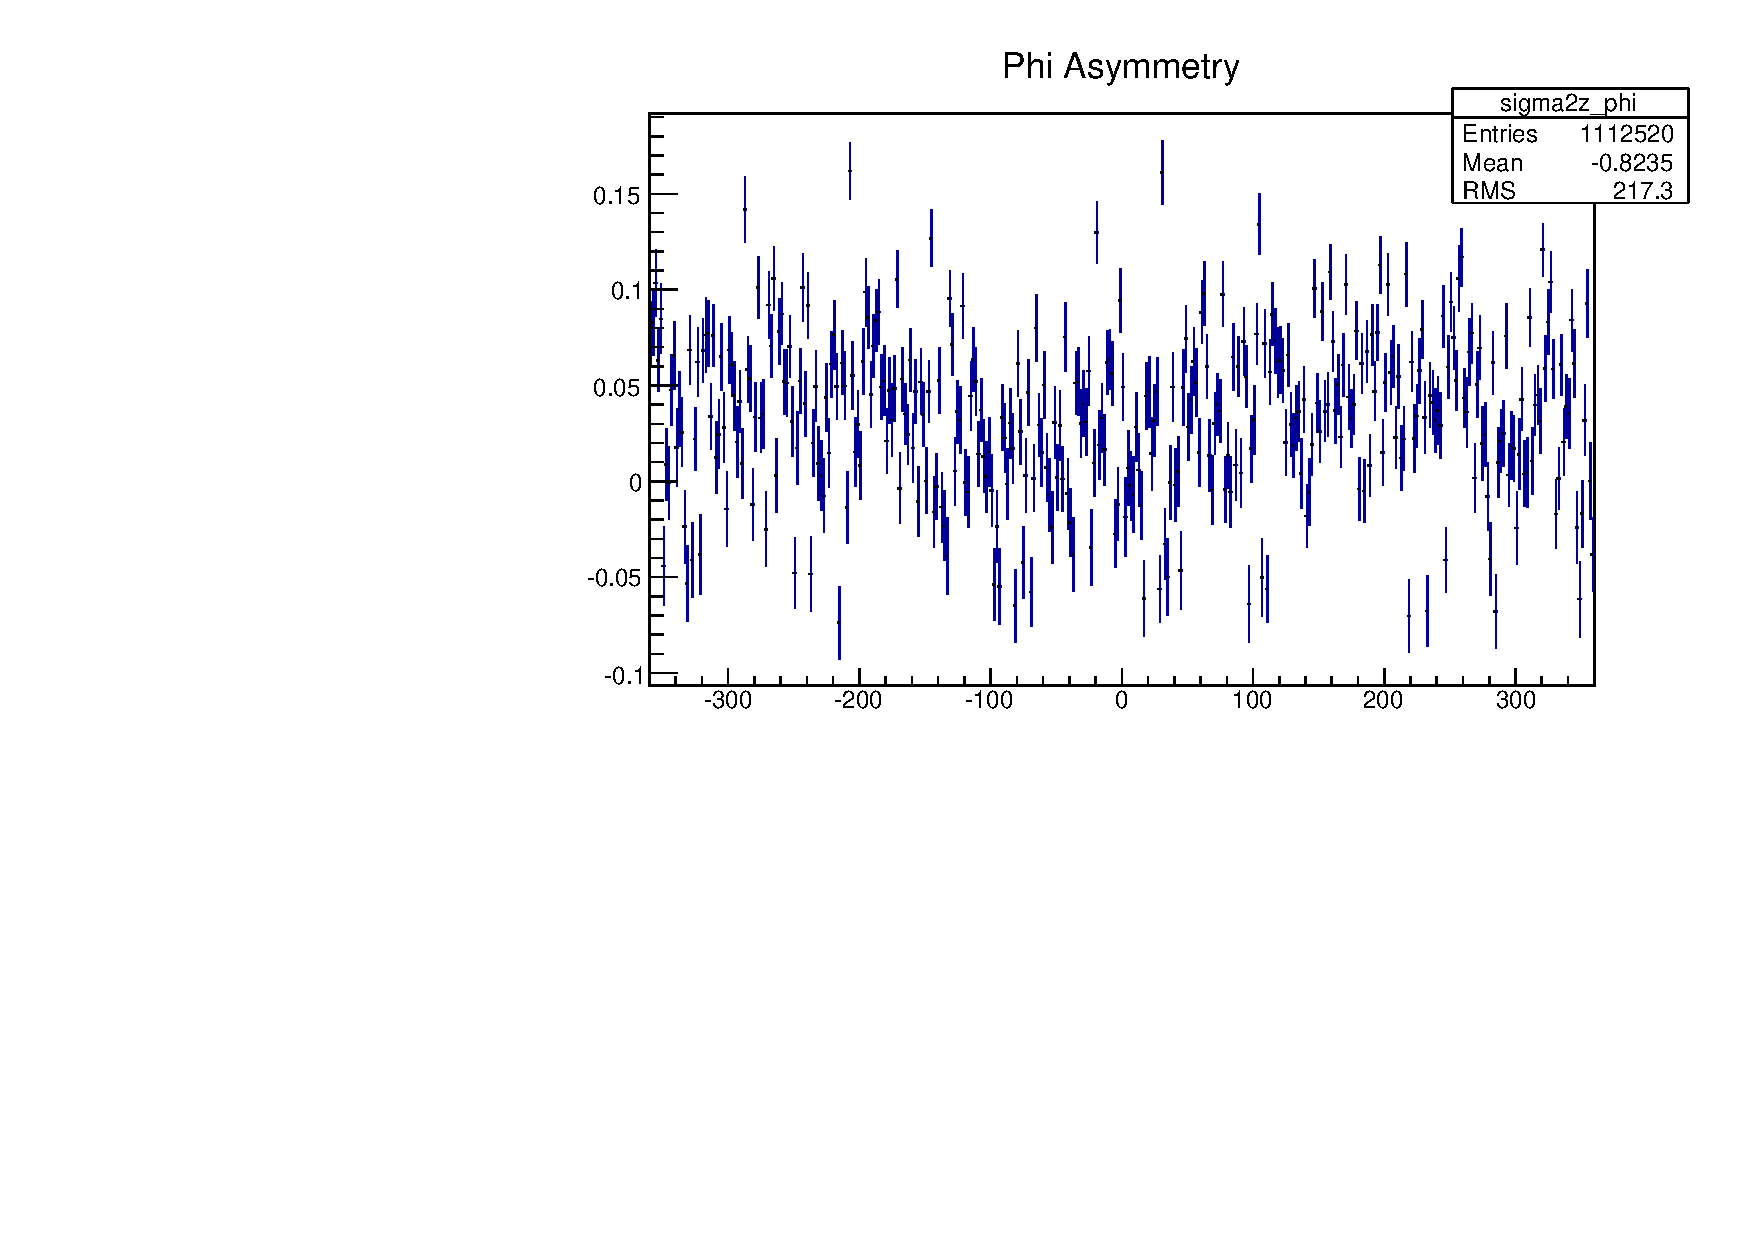
\includegraphics[width=\textwidth]{Asym/phi_asym.pdf}
\caption{Phi asymmetry with no angle cut. }
\end{figure}

\begin{figure}
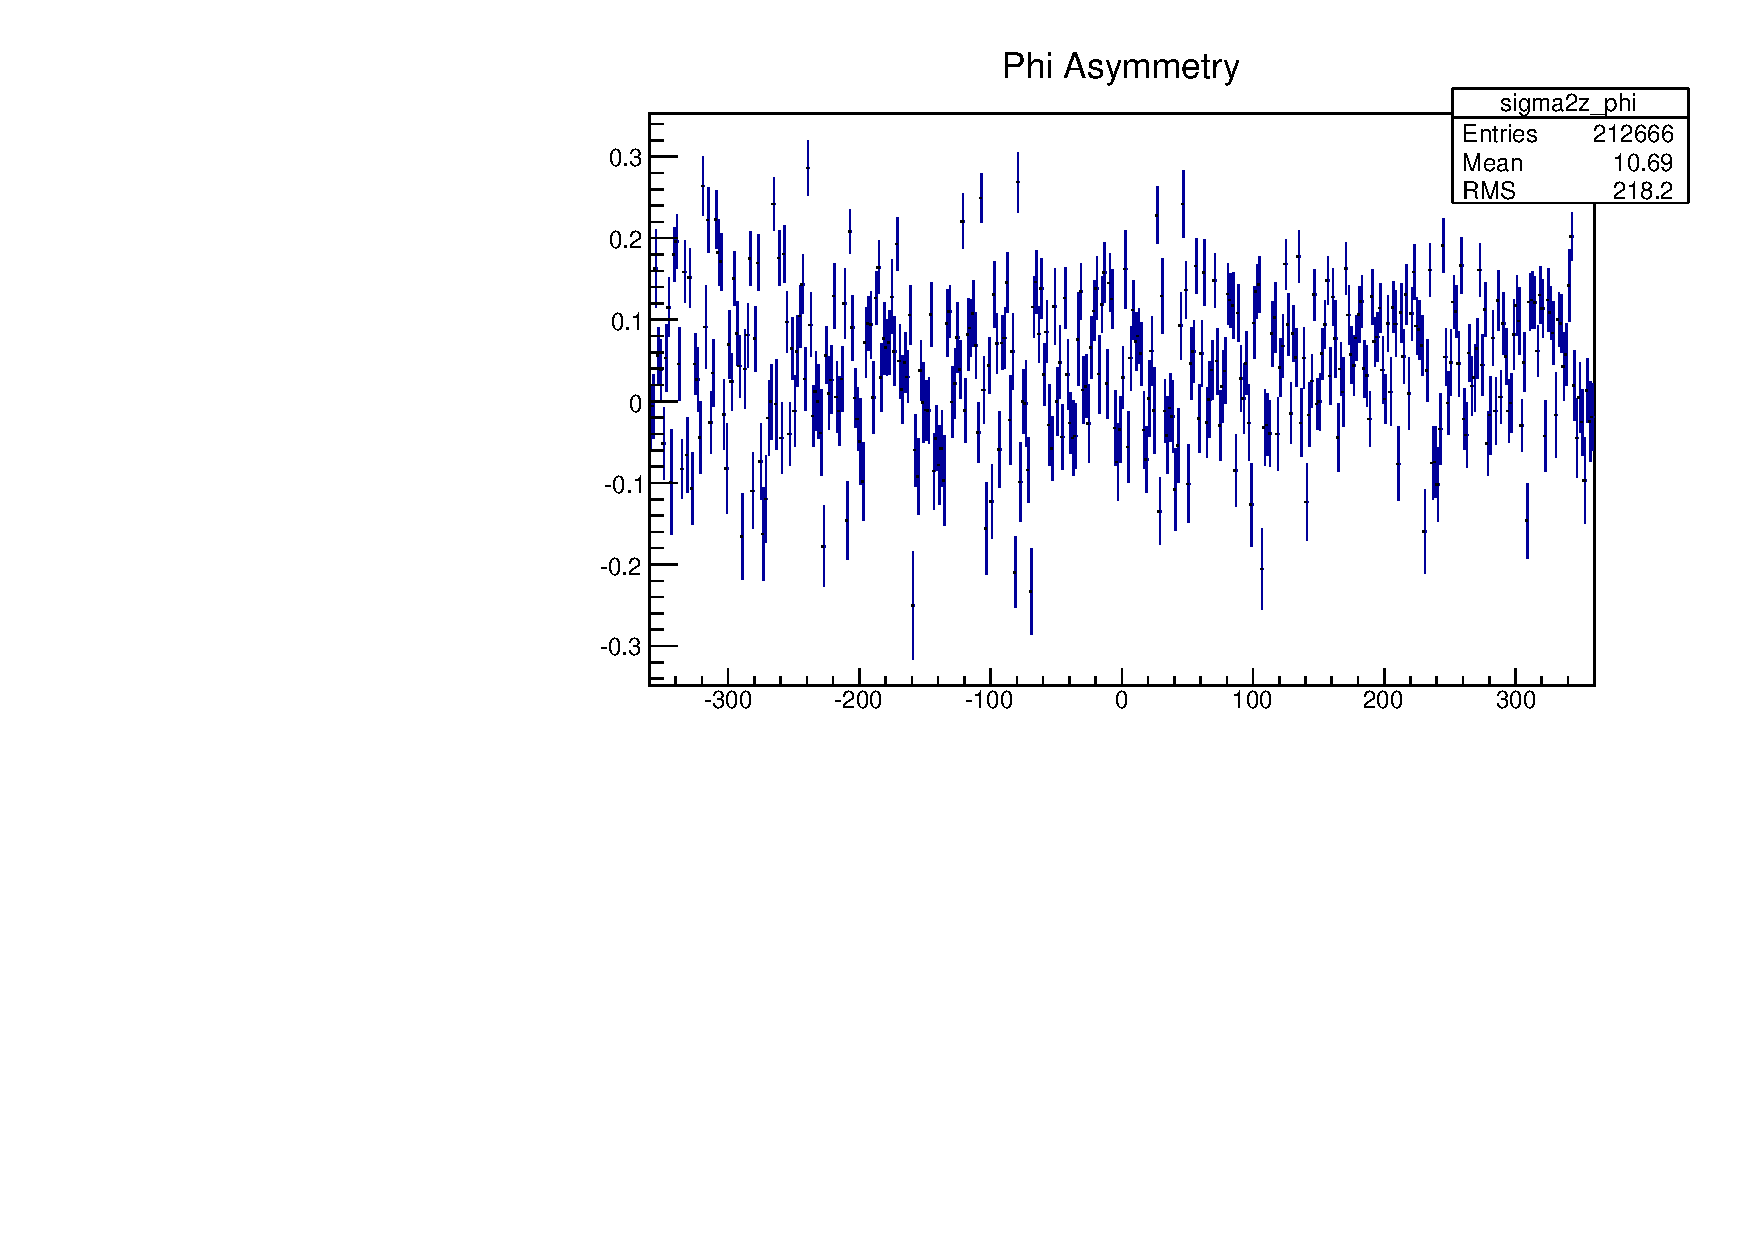
\includegraphics[width=\textwidth]{Asym/phi_asym_thetacut.pdf}
\caption{Phi asymmetry with $100^{\circ} < \theta < 120^{\circ} $ }
\end{figure}


\end{document}
